%%%%%%%%%%%%%%%%%%%%%%%%%%%%%%%%%%%%%%%%%%%%%%%%%%%%%%%%%%%%%%%%%
\documentclass[12pt, a4paper, notitlepage, onecolumn]{article}
\usepackage[UKenglish]{babel}                   % UK style
\usepackage[utf8]{inputenc}
\usepackage[margin=1in]{geometry}               % Margin size
\usepackage{hyperref}                           % Coloured hyperlinks
  \hypersetup{colorlinks = true}
\usepackage{lmodern}                            % Modern fonts
\usepackage{graphicx}                           % For figures
\usepackage[percent]{overpic}                   % For figures with text overlay
\usepackage{amsmath,amssymb}                    % Mathematical symbols
\usepackage{mathtools}
\usepackage{siunitx}                            % SI-units
%\sisetup{exponent-product = \cdot}             % Dot product instead of cross product
\sisetup{separate-uncertainty = true}           % Plus-minus uncertainty
\usepackage{physics}                            % Elegant equations in physics
\usepackage{booktabs}                           % Nice lines, for instance in tables
\usepackage[font=small,labelfont=bf]{caption}% Caption
\usepackage{float}                              % Table do not move with [H].
\usepackage{subcaption}                         % For subfigures
\usepackage[en-GB]{datetime2}                   % UK date format
\usepackage{listings}                           %Source code
\usepackage{feynmp}                             % Feynman diagrams
\DeclareGraphicsRule{*}{mps}{*}{}               % Include Feynman diagrams
\usepackage{scalerel}
\newcommand{\mylbrace}[2]{\vspace{#2pt}\hspace{6pt}\scaleleftright[\dimexpr5pt+#1\dimexpr0.06pt]{\lbrace}{\rule[\dimexpr2pt-#1\dimexpr0.5pt]{-4pt}{#1pt}}{.}}
\newcommand{\myrbrace}[2]{\vspace{#2pt}\scaleleftright[\dimexpr5pt+#1\dimexpr0.06pt]{.}{\rule[\dimexpr2pt-#1\dimexpr0.5pt]{-4pt}{#1pt}}{\rbrace}\hspace{6pt}}
\usepackage{xspace}                             % Fancy LHCb symbols
\usepackage{upgreek}
\def\pythia{\mbox{\textsc{Pythia}}\xspace}
\def\evtgen{\mbox{\textsc{EvtGen}}\xspace}
\def\photos{\mbox{\textsc{Photos}}\xspace}
%\usepackage{natbib}                      % Set line spacing in references
%\setlength{\bibsep}{1.0pt}
%\setcitestyle{square}

\newcommand*{\diff}{\mathrm{d}}

\usepackage[switch]{lineno}

%%%%%%%%%%%%%%%%%%%%%%%%%%%%%%%%%%%%%%%%%%%%%%%%%%%%%%%%%%%%%%%
\title{Model-independent measurement of the CKM angle $\gamma$ in $B^\pm\to[K^+K^-\pi^+\pi^-]_Dh^\pm$ decays}
\author{Martin Duy Tat}
\date{\today}
%\numberwithin{equation}{section}
%%%%%%%%%%%%%%%%%%%%%%%%%%%%%%%%%%%%%%%%%%%%%%%%%%%%%%%%%%%%%%%
\begin{document}
\maketitle
\begin{abstract}
\noindent A model-independent measurement of the CKM angle $\gamma$ is performed in $B^\pm\to Dh^\pm (h = K, \pi)$ decays, where $D\to K^+K^-\pi^+\pi^-$, using the LHCb Run\,$1$+$2$ dataset. The measurement performed in bins of phase space, which are optimised for sensitivity to local $C\!P$ asymmetries. The analysis requires external charm strong-phase inputs, which are determined from quantum-correlated $D\bar{D}$ pairs at BESIII.
\end{abstract}

%%%%%%%%%%%%%%%%%%%%%%%%%%%%%%%%%%%%%%%%%%%%%%%%%%%%%%%%%%%%%%%
\section{Introduction}
\noindent The Standard Model (SM) description of charge-parity ($C\!P$) violation can be tested by measuring the lengths and angles of the Unitary Triangle, which is a geometrical representation of the Cabibbo–Kobayashi–Maskawa quark-mixing matrix~\cite{Kobayashi:1973fv}. In particular, the $C\!P$-violating phase  $\gamma\equiv\arg(-V_{ud}V_{ub}^*/V_{cd}V_{cb}^*)$ is the only angle that can be measured at tree level with negligible theoretical uncertainties~\cite{Brod_2014}. Therefore, it makes an excellent SM benchmark that can be compared with other indirect measurements of $\gamma$ that are more likely to be affected by New Physics.

A powerful decay channel for the measurement of $\gamma$ is $B^\pm\to DK^\pm$, which proceeds through both a favoured $b\to c\bar{u}s$ and a suppressed $b\to u\bar{c}s$ transition. Fig. \ref{fig_feynman_B2DK} shows the $B^-\to D^0K^-$ mode and the colour suppressed $B^-\to\bar{D^0}K^-$ channel, and they interfere when $D^0$ and $\bar{D^0}$ decay to a common state. The interference effects are sensitive to $\gamma$, which can in general be determined from measurements of the appropriate $C\!P$ asymmetries and related observables. This strategy has been pursued for a wide range of $D$ final states at LHCb~\cite{LHCb-PAPER-2021-033}. Effects from $C\!P$-violation also occur in the process $B^\pm\to D\pi^\pm$ through the interference of $b\to c\bar{u}d$ and $b\to u\bar{c}d$ transitions, but these are in general significantly smaller in magnitude.

\begin{figure}[H]
  \centering
  \vspace{0.3cm}
  \begin{subfigure}{0.5\textwidth}
    \centering
    \begin{fmffile}{fgraph/fgraph_BtoDK1}
      \setlength{\unitlength}{0.4cm}
      \begin{fmfgraph*}(8.5,4.5)
        \fmfstraight
        \fmfleft{i1,B,i2,t1,t2,t3,t9,t10}
        \fmfright{o1,D,o2,t4,t5,o3,K,o4}
        \fmflabel{$\bar{u}$}{i1}
        \fmflabel{$b$}{i2}
        \fmfv{l.d=20,l.a=180,l={$B^-$\mylbrace{30}{-8}}}{B}
        \fmflabel{$\bar{u}$}{o1}
        \fmflabel{$c$}{o2}
        \fmflabel{$\bar{u}$}{o3}
        \fmflabel{$s$}{o4}
        \fmfv{l.d=15,l.a=0,l={\myrbrace{34}{-11}}$D^0$}{D}
        \fmfv{l.d=15,l.a=0,l={\myrbrace{32}{6}}$K^-$}{K}
        \fmf{fermion}{o1,i1}
        \fmf{fermion,tension=1.5}{i2,v1}
        \fmf{fermion}{v1,o2}
        \fmf{phantom,tension=1.5}{t9,v2}
        \fmf{boson,label=$W$,label.side=left,tension=0}{v1,v2}
        \fmf{fermion}{v2,o4}
        \fmf{fermion}{o3,v2}
      \end{fmfgraph*}
    \end{fmffile}
    \vspace{0.5cm}
  \end{subfigure}%
  \begin{subfigure}{0.5\textwidth}
    \centering
    \begin{fmffile}{fgraph/fgraph_BtoDK2}
      \setlength{\unitlength}{0.4cm}
      \begin{fmfgraph*}(8.5,4.5)
        \fmfstraight
        \fmfleft{i1,t1,t2,B,t9,t10,i2}
        \fmfright{o1,K,o2,t4,t5,o3,D,o4}
        \fmflabel{$\bar{u}$}{i1}
        \fmflabel{$b$}{i2}
        \fmfv{l.d=20,l.a=180,l={$B^-$\mylbrace{85}{-3}}}{B}
        \fmflabel{$\bar{u}$}{o1}
        \fmflabel{$s$}{o2}
        \fmflabel{$\bar{c}$}{o3}
        \fmflabel{$u$}{o4}
        \fmfv{l.d=15,l.a=0,l={\myrbrace{34}{11}}$\bar{D^0}$}{D}
        \fmfv{l.d=15,l.a=0,l={\myrbrace{35}{-12}}$K^-$}{K}
        \fmf{fermion}{o1,i1}
        \fmf{fermion,tension=1.5}{i2,v1}
        \fmf{fermion}{v1,o4}
        \fmf{phantom,tension=1.5}{t2,v2}
        \fmf{boson,label=$W$,label.side=right,tension=0}{v1,v2}
        \fmf{fermion}{v2,o2}
        \fmf{fermion}{o3,v2}
      \end{fmfgraph*}
    \end{fmffile}
    \vspace{0.5cm}
  \end{subfigure}
  \caption{Feynman diagrams of $B^-\to DK^-$ decays at tree level.}
  \label{fig_feynman_B2DK}
\end{figure}

An interesting class of $D$ final states are self-conjugate multi-body $D$ decays. Since the strong-phase difference between the $D^0$ and $\bar{D^0}$ decays varies across the multi-dimensional phase space of the charm-meson decay, the sensitivity to $\gamma$ is diluted when considering the decay inclusively. However, by performing measurements in localised regions of phase space, the dilution effects can be minimised and the sensitivity to $\gamma$ enhanced~\cite{BondarPoluektov2008,GiriGrossmanSofferZupan}.

The channel $D\to K^+K^-\pi^+\pi^-$ has been proposed as a promising decay mode for measuring $\gamma$~\cite{cite:RademackerWilkinson}. It has a rich resonance structure and contains only charged particles in the final state, which is advantageous for experiments at a hadron collider. The availability of a detailed amplitude model for this process, based on an amplitude analysis of LHCb data~\cite{LHCb-PAPER-2018-041}, opens up the possibility of identifying those regions of phase space that have high sensitivity to $\gamma$, which then can be probed in an analysis of $B^\pm\to DK^\pm$ decays.

The interpretation of the $C\!P$ asymmetries and other observables in these regions, also known as bins of phase space, requires knowledge of the strong-phase difference between the $D^0$ and $\bar{D^0}$ meson decays. This knowledge can be obtained from the same amplitude model used to guide the measurements, but it is preferable to perform a direct measurement at BESIII, using quantum-correlated charm decays at the $\psi(3770)$ resonance. This approach ensures that the determination of $\gamma$ has no dependence on model assumptions. 

Binned strong-phase measurements have previously been done in other decay modes~\cite{LHCb-PAPER-2020-019}, but no such measurement for $D^0\to K^+K^-\pi^+\pi^-$ exists yet. Not only would such a measurement complement the current measurements of $\gamma$, but it would also be crucial information for future studies of $D^0$-$\bar{D^0}$ oscillations and charm $C\!P$ violation.

In this thesis report, the measurement of $\gamma$ in $B^\pm\to[K^+K^-\pi^+\pi^-]_Dh^\pm$, using data from LHCb and BESIII, is presented. An optimised five-dimensional binning scheme is developed for this measurement. At BESIII, an inclusive phase space analysis of $D^0\to K^+K^-\pi^+\pi^-$ is first performed, and the strategies for expanding this strong-phase analysis into bins of phase space is described. Finally, the $B^\pm\to[K^+K^-\pi^+\pi^-]_Dh^\pm$ decay is studied at LHCb, using model-predicted strong-phase inputs. When the BESIII analysis is completed in the near future, the LHCb result may be readily updated, which will result in the first measurement of $\gamma$ in this channel.

%%%%%%%%%%%%%%%%%%%%%%%%%%%%%%%%%%%%%%%%%%%%%%%%%%%%%%%%%%%%%%%
\section{Formalism}
\subsection{Strong-phase inputs from quantum-correlated \texorpdfstring{\boldmath{$D^0\bar{D^0}$}}{DD} decays}
\noindent The formalism described in this Section closely follows that of Ref.~\cite{HarnewS4pi}. In charm factories, charm mesons are produced in $e^+e^-$ collisions at the $\psi(3770)$ resonance. The strong decay of $\psi(3770)\to D\bar{D}$ conserves the $C = -1$ quantum number of the initial state, leaving the $D$-meson pair in an anti-symmetric wave function. This quantum correlation allows for a direct access to the strong-phase difference between $D^0$ and $\bar{D^0}$ decays through a double-tag (DT) analysis. The method uses single-tag (ST) events, which are events where only one of the charm mesons is reconstructed, with no requirements on the decay of the other meson, and DT events, where both $D$ mesons are reconstructed, one in a tag mode and the other in the signal mode $D^0\to K^+K^-\pi^+\pi^-$.

In DT events, the phase space of the $D\to K^+K^-\pi^+\pi^-$ decay is split into $2\times\mathcal{N}$ bins, labelled from $i = -\mathcal{N}$ to $i = \mathcal{N}$, excluding zero. Bin $-i$ is related to bin $+i$ by a $C\!P$ transformation. The choice of binning scheme is described in Sec.~\ref{section:Binning_scheme}. When the signal mode is tagged using different tag types, one may infer the strong-phase information by studying the bin yields. These will evolve in a non-trivial manner across different bins due to different strong-phase differences.

Table~\ref{table:Tag_modes} lists all the tag modes used for this analysis. The analysis can be split into four categories: Flavour tags, $C\!P$ tags, $K_S^0\pi^+\pi^-$, and $K_L^0\pi^+\pi^-$. Flavour tags are used to determine the flavour of the charm meson in the signal mode. The $C\!P$ tags are modes in which the $D$ meson decays to a $C\!P$ eigenstate. The modes $D\to K_{S, L}^0\pi^+\pi^-$ are of mixed $C\!P$ content, since these decays can proceed through both $C\!P$-even and $C\!P$-odd amplitudes. The mode $\pi^+\pi^-\pi^0$ is listed as a $C\!P$-even tag since its $C\!P$-even fraction, $F_+^{\pi\pi\pi^0} = 0.973 \pm 0.017$~\cite{cite:pipipi0_CPfraction}, is very close to unity.

\begin{table}[htb]
    \centering
    \caption{Tag modes used in this analysis.}
    \label{table:Tag_modes}
    \begin{tabular}{cc}
        \hline
        Category     & Tag modes \\
        \hline
        Flavour      & $K^-\pi^+$, $K^-\pi^+\pi^0$, $K^-\pi^+\pi^-\pi^+$, $K^-e^+\nu_e$ \\
        $C\!P$ even  & $K^+K^-$, $\pi^+\pi^-$, $K_S^0\pi^0\pi^0$, $\pi^+\pi^-\pi^0$, $K_L^0\pi^0$ \\
        $C\!P$ odd   & $K_S^0\pi^0$, $K_S^0\eta_{\gamma\gamma}$, $K_S^0\eta^\prime(\pi\pi\eta)$, $K_S^0\eta^\prime(\rho^0\gamma)$, $K_S^0\omega$ \\
        Mixed $C\!P$ & $K_S^0\pi^+\pi^-$, $K_L^0\pi^+\pi^-$ \\
        \hline
    \end{tabular}
\end{table}

Events where one $D$ meson is reconstructed as the signal decay $D\to K^+K^-\pi^+\pi^-$, while the other is reconstructed as a flavour tag mode $f$, have no sensitivity to strong phases due to the abscence of quantum correlations. However, such events are useful to determine the fractional bin yield $K_i$ of signal decays into bin $i$. This is given by the ratio of the DT yield $N^{\rm DT}$ and ST yield $N^{\rm ST}$~\cite{HarnewS4pi},

\begin{equation}
    \frac{N^{\rm DT}(KK\pi\pi | f)}{N^{\rm ST}(f)}\times\frac{\epsilon_{\rm ST}(f)}{\epsilon_{\rm DT}(KK\pi\pi | f)} = \mathcal{B}(KK\pi\pi)K_i,
    \label{equation:Flavour_tag_Ki}
\end{equation}
where $\mathcal{B}(KK\pi\pi)$ is the branching fraction of $D^0\to K^+K^-\pi^+\pi^-$ and $\epsilon_{\rm DT(ST)}$ is the reconstruction efficiency of the DT (ST) event.

Instead, if $f$ is reconstructed as a pure or mixed-$C\!P$ tag mode, the predicted ratio of DT to ST yield is\cite{HarnewS4pi}
\begin{equation}
    \frac{N_i^{\rm DT}(KK\pi\pi | f)}{N^{\rm ST}(f)}\times\frac{\epsilon_{\rm ST}(f)}{\epsilon_{\rm DT}(KK\pi\pi | f)} = \mathcal{B}(KK\pi\pi)\big(K_i + K_{-i} - 2\sqrt{K_iK_{-i}}(2F_+^{f} - 1)c_i\big),
    \label{equation:DT_ST_yield_ratio}
\end{equation}
where $F_+^f$ is the $C\!P$-even fraction of the tag mode. For pure $C\!P$-even (odd) tags, $F_+^f = 1$ ($0$). $c_i$ is the cosine of the amplitude-averaged strong-phase difference $\Delta\delta_D = \delta_D(\Phi) - \delta_D(\bar{\Phi})$ of the $D$ decay in bin $i$, given by

\begin{equation}
    c_i\equiv\frac{\int_i\diff\Phi\lvert\mathcal{A}_{D^0}\rvert\lvert\mathcal{A}_{\bar{D^0}}\rvert\cos(\Delta\delta_D)}{\sqrt{\int_i\diff\Phi\lvert\mathcal{A}_{D^0}\rvert^2\int_i\diff\Phi\lvert\mathcal{A}_{\bar{D^0}}\rvert^2}}.
    \label{equation:ci}
\end{equation}
In Eq.~\eqref{equation:ci}, $\mathcal{A}_{D^0}$ is the amplitude of the decay $D^0\to K^+K^-\pi^+\pi^-$ and $\Phi$ labels the position in the five-dimensional phase space. The integral over $\Phi_i$ is performed over the phase-space region that belongs to bin $i$. The $C\!P$-conjugated amplitude $\mathcal{A}_{\bar{D^0}}(\Phi)$ is equal to $\mathcal{A}_{D^0}(\bar{\Phi})$, where $\bar{\Phi}$ is obtained by swapping the charges and momentum directions of the $D$-decay products. The expression for $s_i$, the sine of the $D$ strong-phase difference, is analogous.

For the $K_S^0\pi^+\pi^-$ tag, which is a decay mode of mixed $C\!P$, an enhanced sensitivity to the strong-phase differences is obtained by separating events into bins of phase space of the tag decay as well. Additionally, binning the tag mode provides sensitivity to $s_i$. For the $D^0\to K^0_S\pi^+\pi^-$ decay mode, the fractional yield $K_i^f$ and the amplitude-averaged cosine and sine of the strong-phase difference $c_i^f$ and $s_i^f$ have been measured in each bin~\cite{cite:KSpipiStrongPhase}. The combined CLEO and BESIII results from Ref.~\cite{cite:KSpipiStrongPhase} are used, and they are treated as external inputs. The yield-ratio expression in bin $i$ on the signal side and bin $j$ on the tag side is~\cite{HarnewS4pi}

\begin{linenomath}
    \begin{align}
        \frac{N_{ij}^{\rm DT}(KK\pi\pi | f)}{N^{\rm ST}(f)}&\times\frac{\epsilon_{\rm ST}(f)}{\epsilon_{\rm DT}(KK\pi\pi | f)} = \nonumber \\
        \frac{1}{2}\mathcal{B}(KK\pi\pi)&\big(K_iK_{-j}^f + K_{-i}K_j^f - 2\sqrt{K_iK_{-i}K_j^fK_{-j}^f}c_ic_j^f + s_is_j^f\big).
        \label{equation:DT_ST_yield_ratio_K0pipi}
    \end{align}
\end{linenomath}
The expression for the $D\to K_L^0\pi^+\pi^-$ tag is analogous, but with a sign swap in $c_i^f$ and $s_i^f$, and their values are also reported in Refs.~\cite{cite:KSpipiStrongPhase}.

If the available statistics is insufficient to determine $c_i$ (and $s_i$), it is possible to consider the phase-space of $D^0\to K^+K^-\pi^+\pi^-$ inclusively. This has the disadvantage of diluting the strong-phase differences. Eq.~\eqref{equation:DT_ST_yield_ratio} then simplifies to

\begin{equation}
    \frac{N^{\rm DT}(KK\pi\pi | f)}{N^{\rm ST}(f)}\times\frac{\epsilon_{\rm ST}(f)}{\epsilon_{\rm DT}(KK\pi\pi | f)} = \mathcal{B}(KK\pi\pi)\big(1 - (2F_+^{f} - 1)(2F_+ - 1)\big),
    \label{equation:DT_ST_yield_ratio_FPlus}
\end{equation}
while Eq.~\eqref{equation:DT_ST_yield_ratio_K0pipi} becomes
\begin{equation}
    \frac{N_i^{\rm DT}(KK\pi\pi | f)}{N^{\rm ST}(f)}\times\frac{\epsilon_{\rm ST}(f)}{\epsilon_{\rm DT}(KK\pi\pi | f)} = \mathcal{B}(KK\pi\pi)\big(K_i + K_{-i} - 2\sqrt{K_iK_{-i}}c_i(2F_+ - 1)\big).
    \label{equation:DT_ST_yield_ratio_K0pipi_FPlus}
\end{equation}
For a phase-space inclusive analysis, the strong-phase information is encoded in the $C\!P$-even fraction $F_+$ of the $D^0\to K^+K^-\pi^+\pi^-$ decay. The quantity $2F_+ - 1$ can be identified as the cosine of the amplitude-averaged strong-phase of the whole phase space.

%%%%%%%%%%%%%%%%%%%%%%%%%%%%%%%%%%%%%%%%%%%%%%%%%%%%%%%%%%%%%%%
\subsection{Measurement of \texorpdfstring{\boldmath{$\gamma$}}{gamma} using \texorpdfstring{\boldmath{$B^\pm$}}{B} decays}
\noindent The analysis of $B^\pm\to[K^+K^-\pi^+\pi^-]_Dh^\pm$ to determine $\gamma$ follows the formalism described in Ref.~\cite{LHCb-PAPER-2020-019}. The $B^-\to DK^-$ decay can proceed via the favoured $B^-\to D^0K^-$ amplitude, or via the suppressed $B^-\to\bar{D^0}K^-$ amplitude. The overall amplitude of this decay is a coherent sum of the two decay paths,
\begin{equation}
    \mathcal{A}_B^-(\Phi) = \mathcal{A}_{B^-}^{D^0K^-}\Big(\mathcal{A}_{D^0}(\Phi) + r_B^{DK}\exp\big(i(\delta_B^{DK} - \gamma)\big)\mathcal{A}_{\bar{D^0}}(\Phi)\Big),
    \label{equation:Bpm_amplitude}
\end{equation}
where $\mathcal{A}_{B^-}^{D^0K^-}$ is the amplitude of the favoured $B^-\to D^0 K^-$ decay, $\mathcal{A}_{D^0}$ ($\mathcal{A}_{\bar{D^0}}$) is the amplitude of the $D^0$ ($\bar{D^0}$) decay, $r_B^{DK}$ is the magnitude of the ratio of the $B$-decay amplitudes, $\delta_B^{DK}$ is the strong-phase difference of the amplitudes and $\gamma$ is the weak-phase. The corresponding expression for the $B^+$ decay is obtained by making the substitutions $\gamma\to -\gamma$ and $\mathcal{A}_{D^0}\to\mathcal{A}_{\bar{D^0}}$.

The expected yield of $B^-$ decays in bin $i$ is obtained by integrating Eq.~\eqref{equation:Bpm_amplitude}, and the corresponding expression for $B^+$ decays. Defining the $C\!P$-violating observables

\begin{equation}
    x_\pm^{DK} = r_B^{DK}\cos(\delta_B^{DK}\pm\gamma), \quad y_\pm^{DK} = r_B^{DK}\sin(\delta_B^{DK}\pm\gamma),
    \label{equation:CP_observables}
\end{equation}
the yields $N_i^\pm$ of $B^\pm$ candidates in bin $i$ are given by 
\begin{align}
    N_{+i}^+ &= h_{B^+}^{DK}\Big(F_{-i} + \big((x_+^{DK})^2 + (y_+^{DK})^2\big)F_{+i} + 2\sqrt{F_{+i}F_{-i}}\big(x_+^{DK}c_i - y_+^{DK}s_i\big)\Big), \label{equation:Ni_plus} \\
    N_{-i}^- &= h_{B^-}^{DK}\Big(F_{-i} + \big((x_-^{DK})^2 + (y_-^{DK})^2\big)F_{+i} + 2\sqrt{F_{+i}F_{-i}}\big(x_-^{DK}c_i - y_-^{DK}s_i\big)\Big), \label{equation:Ni_minus}
\end{align}
where $h_{B^\pm}^{DK}$ are normalisation constants. Since $h_{B^+}^{DK}$ and $h_{B^-}^{DK}$ are independent fit parameters, the binned measurement is insensitive to the $B^\pm$ production asymmetry and any charge asymmetry in the detection efficiency of the kaon that accompanies the $D$ meson.

Equations~\eqref{equation:Ni_plus} and \eqref{equation:Ni_minus} are sensitive to $\gamma$ through the interference terms, and the magnitude of the interference is determined by the size of $r_B^{DK}$, which has been measured to be $\approx 0.1$~\cite{LHCb-PAPER-2021-033}. The parameters $F_i$ are defined as
\begin{equation}
    F_i\equiv\frac{\int_i\diff\Phi\eta(\Phi)\lvert\mathcal{A}_{D^0}\rvert^2}{\int\diff\Phi\eta(\Phi)\lvert\mathcal{A}_{D^0}\rvert^2},
    \label{equation:Fi}
\end{equation}
which are analogous to $K_i$, but contains the function $\eta(\Phi)$ to account for the experimental acceptance, which in general depends on the location of the decay in phase space.

Analogous expressions to Eqs.~\ref{equation:CP_observables},~\ref{equation:Ni_plus} and~\ref{equation:Ni_minus} can be written for the decay mode $B^\pm\to D\pi^\pm$, with the $DK$ superscripts replaced by $D\pi$. Since the decay topology is identical to that of $B^\pm\to DK^\pm$, the phase-space acceptance $\eta(\Phi)$ is expected to be very similar between the two $B^\pm$-decay modes, and studies using simulation samples show that any differences are negligible within the current precision. Thus, the $F_i$ parameters can be considered as common between $B^\pm\to D\pi^\pm$ and $B^\pm\to DK^\pm$ decays. The mode $B^\pm\to D\pi^\pm$ has a branching fraction that is an order of magnitude larger than that of the $B^\pm\to DK^\pm$ mode, but the interference effects, governed by the parameter $r_B^{D\pi}\approx 0.005$~\cite{LHCb-PAPER-2021-033}, are much smaller. Therefore, this decay has a significantly lower sensitivity to $\gamma$, but is a suitable mode for determining the $F_i$ parameters. By including the $B^\pm\to D\pi^\pm$ channel as a signal mode, the $F_i$ can be treated as free parameters in the analysis, thus form of the acceptance function $\eta(\Phi)$ is not needed.

From the definition of Eq.~\eqref{equation:Fi}, it follows that $\sum_iF_i = 1$. Therefore, only $2\mathcal{N} - 1$ of the $F_i$ parameters are independent. To accommodate this constraint in the analysis, the $F_i$ parameters are fitted with the alternative parameterisation

\begin{equation}
    F_i =
    \begin{cases}
        R_i, & i = -N \\
        R_i\prod_{j < i}(1 - R_j), & -N < i < +N \\
        \prod_{j < i}(1 - R_j), &i = +N.
    \end{cases}
\end{equation}
%\vspace*{0.2cm}
Measuring the yields of $B^\pm$ decays in each bin of phase space allows the eight $C\!P$-violating observables $x_\pm^{DK}$, $y_\pm^{DK}$, $x_\pm^{D\pi}$ and $y_\pm^{D\pi}$ to be determined. These $C\!P$-violating observables can be interpreted in terms of the five underlying physics parameters $\gamma$, $\delta_B^{DK}$, $r_B^{DK}$, $\delta_B^{D\pi}$ and $r_B^{D\pi}$.

Studies performed with pseudoexperiments demonstrate that a fit where all eight $C\!P$-violating observables are free parameters is unstable for $r_B^{D\pi} < 0.03$, due to large correlations between the $B^\pm\to D\pi^\pm$ $C\!P$-violating observables and the $F_i$ parameters~\cite{LHCb-PAPER-2020-019}. Since $\gamma$ is a common parameter between the $B^\pm\to DK^+$ and $B^\pm\to D\pi^+$ analyses, the $C\!P$-violating observables for the $B^\pm\to D\pi^+$ mode can be re-parameterised as

\begin{equation}
    x_\xi^{D\pi} = \Re\big(\xi^{D\pi}\big), \quad y_\xi^{D\pi} = \Im\big(\xi^{D\pi}\big), \quad \xi^{D\pi} = \frac{r_B^{D\pi}}{r_B^{DK}}\exp\Big(i\big(\delta_B^{D\pi} - \delta_B^{DK}\big)\Big).
\end{equation}

In summary, a measurement of the bin yields of $B^\pm\to[K^+K^-\pi^+\pi^-]_D h^\pm$ decays in bins of phase space allows the six $C\!P$-violating observables $x_\pm^{DK}$, $y_\pm^{DK}$, $x_\xi^{D\pi}$ and $y_\xi^{D\pi}$ to be determined, along with the experiment-specific parameters $F_i$, expressed in terms of $R_i$, and the four normalisation parameters $h_{B^\pm}^{D h}$.

%%%%%%%%%%%%%%%%%%%%%%%%%%%%%%%%%%%%%%%%%%%%%%%%%%%%%%%%%%%%%%%
\subsection{Binning scheme}
\label{section:Binning_scheme}
In the $B^\pm\to DK^\pm$, $D\to K^0_S h^+h^-$ ($h=\pi, K$) analysis presented in Ref.~\cite{LHCb-PAPER-2020-019}, an optimal binning scheme, that can be visualised in a two-dimensional Dalitz plot, is used to maximise the sensitivity to $\gamma$. The binning scheme for the $D^0\to K^+K^-\pi^+\pi^-$ decay is defined analogously, but cannot be easily visualised, as the phase space of four-body decays is five-dimensional.

When defining a binning scheme for the decay $D\to K^+K^-\pi^+\pi^-$, there are two main requirements. Firstly, it should minimise the dilution of the strong phases when averaged over each bin. Secondly, it should maximise the interference effects and thus the sensitivity to $\gamma$. The scheme is constructed with the guidance   of the amplitude model presented in Ref.~\cite{LHCb-PAPER-2018-041}.
 
The position of a $D$ decay in phase space is specified by the four-momenta of the decay products.  These four-momenta allow the corresponding decay amplitudes $\mathcal{A}_{D^0}$ and $\mathcal{A}_{\bar{D^0}}$ of the $D^0$ and $\bar{D^0}$ decays, respectively, to be determined from the amplitude model.  From the $D^0$ and $\bar{D^0}$ decay amplitudes, two convenient parameters,

\begin{equation}
    \Delta\delta_D\equiv\arg\Big(\frac{\mathcal{A}_{D^0}}{\mathcal{A}_{\bar{D^0}}}\Big), \quad r_D\equiv\Big\lvert\frac{\mathcal{A}_{D^0}}{\mathcal{A}_{\bar{D^0}}}\Big\rvert,
\end{equation}
are defined. These are the strong-phase difference and the magnitude of the ratio between the $D^0$ and $\bar{D^0}$ amplitudes according to the model, respectively. Effectively, by considering $\Delta\delta_D$ and $r_D$ as parameters, each $D$ decay in the five-dimensional phase space is projected onto a two-dimensional surface, where a binning scheme can be defined.

The binning is first performed in the $\Delta\delta_D$ coordinate, which spans the range $[-\pi, \pi]$ and is divided into $\mathcal{N}$ bins with boundaries that are symmetric around $\Delta\delta_D=0$. Assigning a decay to such a bin ensures it is grouped with other decays with a similar strong-phase difference, which minimises the dilution in sensitivity to $\gamma$. Bin $i$ is then divided in two, with labels $i$ and $-i$ according to the value of $r_{D}$, giving $2 \times {\mathcal N}$ bins in total. This division is performed in a manner to enhance the difference between $F_{+i}$ and $F_{-i}$, which maximises the magnitude of the interference terms in Eqs.~\eqref{equation:Ni_plus} and \eqref{equation:Ni_minus}. Candidates with $\ln r_D < 0$ ($> 0$) are assigned to bin $i > 0$ ($< 0$), and the bin numbering starts at $i = \mathcal{N}$ ($i = 1$) near $\Delta\delta_D = -\pi$, with decreasing (increasing) bin numbers.

Following the procedure described in Ref.~\cite{HarnewS4pi}, the binning scheme is optimised by adjusting the bin boundaries in $\Delta \delta_D$ to maximise the $Q$-value, 
 defined as $Q^2 = (Q_+^2 + Q_-^2)/2$, where
\begin{equation}
    Q_\pm^2 = 1 - \Big(1 - \sum_i\frac{F_iF_{-i}\big(1 - c_i^2 - s_i^2\big)}{N_{i}^\pm}\Big)\Big(\sum_iF_i\Big)^{-1}.
    \label{equation:Qvalue}
\end{equation}
Here $N_i^\pm$, the $B^\pm \to DK^\pm$ decay yield in bin $i$, as predicted by Eqs.~\eqref{equation:Ni_plus} and~\eqref{equation:Ni_minus}, is calculated with the normalisation coefficients $h_{B^\pm}$ set to unity. The parameters $Q_{\pm}$ give the statistical sensitivity of $x_\pm$ and $y_\pm$ from a binned fit, divided by that of an unbinned fit. With an infinite number of bins, $Q\to 1$. This metric neglects any perturbation to the sensitivity that may arise from the presence of background events.

Only even values of $\mathcal{N}$ are considered and the bin boundaries at $\Delta\delta_D = 0$ and $\pm\pi$ are fixed. Then each pair of bin boundaries on either side of $\Delta\delta_D = 0$ are adjusted until the $Q$-value is maximal. In each iteration $F_i$, $c_i$ and $s_i$  are calculated from the amplitude model using Eqs.~\eqref{equation:ci} and~\eqref{equation:Fi}, assuming a uniform acceptance. The five-dimensional integral over phase space is performed with Monte Carlo integration. Large samples of $D$-decays are generated for the integration, such that the uncertainty due to the finite sample size is negligible. The values of $N_i^\pm$ are determined from Eqs.~\eqref{equation:Ni_plus} and \eqref{equation:Ni_minus}, and take as input $\gamma = 75^\circ$, $\delta^{DK}_B = 130^\circ$ and $r^{DK}_B = 0.1$, which lie close to the known values of these parameters~\cite{LHCb-PAPER-2021-033}. Note, however, that $Q$ has a very weak dependence on the values of the phases assumed in these expressions, and so this choice does not bias the analysis.

Figure~\ref{figure:Binning_scheme_plot_8bins} shows the binning scheme resulting from this procedure for $2 \times 8$ bins, and the values of $c_i$ and $s_i$ predicted by the amplitude model are shown in Fig.~\ref{figure:ci_si_2x8}. In the calculation, the region of phase space where the $\pi^+\pi^-$ invariant mass lies close to the $K^0_S$ mass is excluded. This requirement, which removes around $5\%$ of signal decays, matches the selection requirement that removes $K^0_S\to\pi^+\pi^-$ background, described in Sec.~\ref{section:Candidate_selection}.

The binning scheme shown in Fig.~\ref{figure:Binning_scheme_plot_8bins} has $Q = 0.90$, which indicates that only $10\%$ of the statistical sensitivity is lost through the binning of phase space.

\begin{figure}[htb]
    \centering
    \begin{subfigure}{0.57\textwidth}
        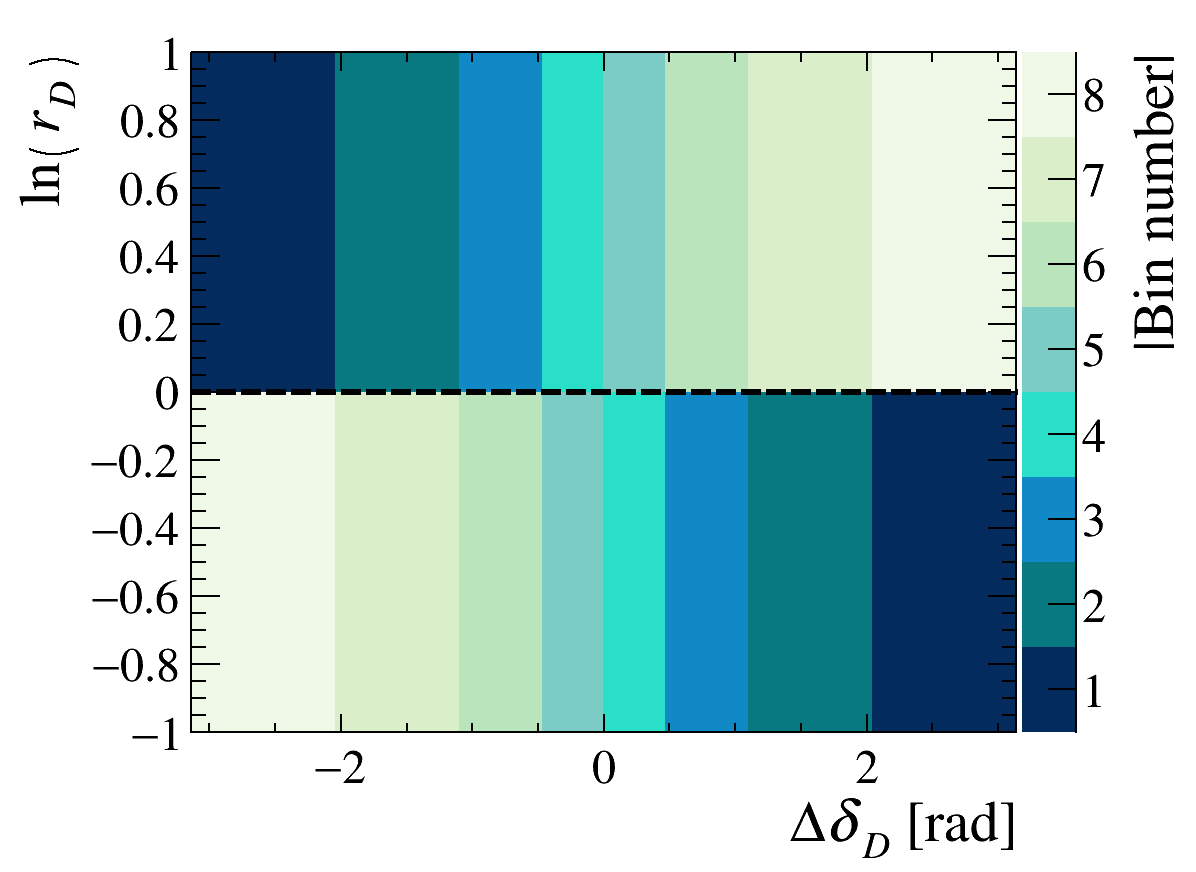
\includegraphics[height=6.2cm]{Plots/BinningSchemePlot_8Bins.png}
        \caption{}
        \label{figure:Binning_scheme_plot_8bins}
    \end{subfigure}%
    \hfill
    \begin{subfigure}{0.43\textwidth}
        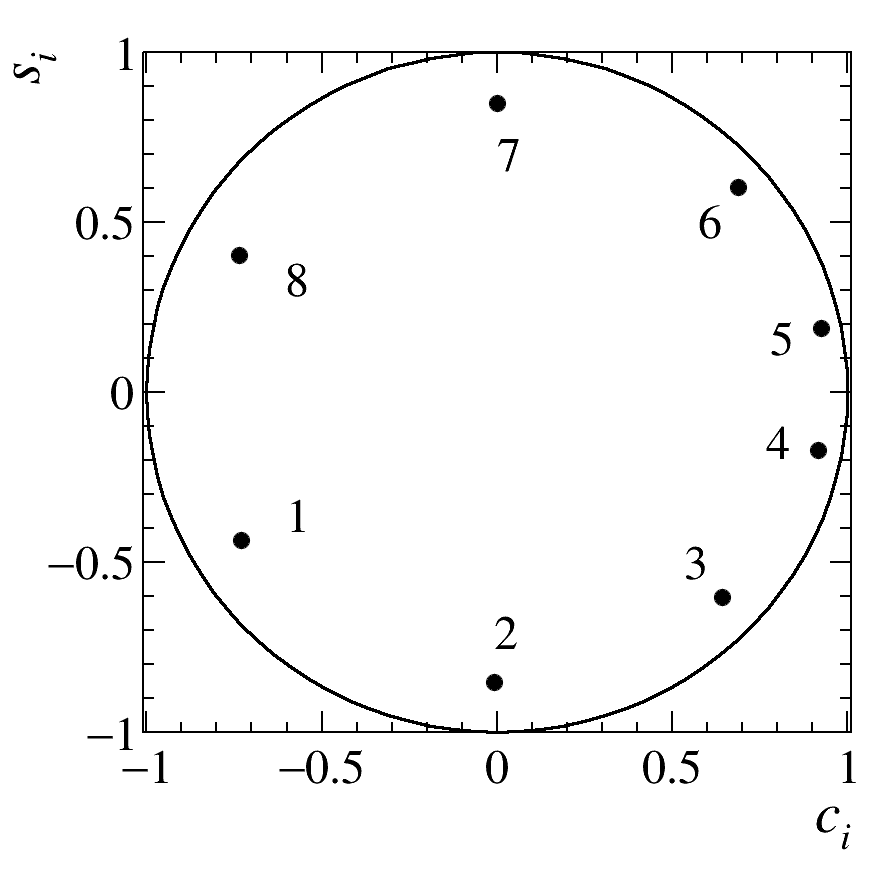
\includegraphics[height=6.2cm]{Plots/StrongPhaseParametersPlot_cisi_8Bins.png}
        \caption{}
        \label{figure:ci_si_2x8}
    \end{subfigure}
    \caption{The optimised $2\times 8$ binning scheme in $\Delta \delta_D$-$\ln(r_D)$ space (left) and the associated $c_i$ and $s_i$ parameters calculated using the amplitude  model (right). The numbers indicate the bin numbers.}
    \label{figure:Binning_scheme_plots_8bins}
\end{figure}

%%%%%%%%%%%%%%%%%%%%%%%%%%%%%%%%%%%%%%%%%%%%%%%%%%%%%%%%%%%%%%%
\section{Analysis of \texorpdfstring{\boldmath{$D^0\to K^+K^-\pi^+\pi^-$}}{D2KKpipi} at BESIII}
\subsection{The BESIII detector}
\noindent BESIII \cite{Ablikim:2009aa} is a general purpose solenoidal detector. The parts most relevant to this analysis are the Helium Multilayer Drift Chamber (MDC) for measuring the momenta and $\dd{E}/\dd{x}$ of charged particles, a Time Of Flight (TOF) system for particle ID and an ElectroMagnetic Calorimeter (EMC) to measure shower energies. The dataset currently under consideration, collected in 2010-2011, has $\SI{2.9}{\per\femto\barn}$ of $e^+e^-\to\psi(3770)$ events, but this will grow to $\SI{20}{\per\femto\barn}$ by the end of 2024~\cite{cite:BESIIIWhitePaper}. Part of this larger dataset has already been collected during 2022 and will be ready for analysis in the near future.

%%%%%%%%%%%%%%%%%%%%%%%%%%%%%%%%%%%%%%%%%%%%%%%%%%%%%%%%%%%%%%%
\subsection{Single- and double-tag reconstruction}
\noindent In the BESIII detector, neutral $D$-meson decays are reconstructed from charged tracks or neutral showers. Charged tracks detected in the MDC are required to be within a polar angle ($\theta$) range of $|\!\cos\theta|<0.93$, where $\theta$ is defined with respect to the $z$-axis, which is the symmetry axis of the MDC. For charged tracks not originating from $K_S^0$ decays, the distance of closest approach to the interaction point (IP), $|V_{z}|$, must be less than 10\,cm along the $z$-axis, and less than 1\,cm in the transverse plane.

Photon candidates are identified using showers in the EMC. The deposited energy of each shower must be more than 25~MeV in the barrel region ($|\cos \theta|< 0.80$) and more than 50~MeV in the end-cap region ($0.86 <|\!\cos \theta|< 0.92$). To exclude showers that originate from charged tracks, the angle subtended by the EMC shower and the position of the closest charged track at the EMC must be greater than 10 degrees as measured from the IP. To suppress electronic noise and showers unrelated to the event, the difference between the EMC time and the event-start time is required to be within [0, 700]\,ns.

Particle identification~(PID) for charged tracks combines measurements of d$E$/d$x$ in the MDC, and time of flight as measured by the TOF system, to form likelihoods $\mathcal{L}(h)$ for each hadron hypothesis $h$. Kaons and pions are identified by comparing the likelihoods for the kaon and pion hypotheses, $\mathcal{L}(K)>\mathcal{L}(\pi)$ and $\mathcal{L}(\pi)>\mathcal{L}(K)$, respectively.

Each $K_{S}^0$ candidate is reconstructed from two oppositely charged tracks satisfying $|V_{z}|<$ 20~cm. The two charged tracks are assigned the pion hypothesis without imposing PID criteria. They are constrained to originate from a common vertex and are required to have an invariant mass within 12~MeV$/c^{2}$ of the known $K^0_{S}$ mass~\cite{pdg}. The $K^0_S$ decay length is required to be greater than twice the vertex resolution away from the IP.

Candidate $\pi^0$ and $\eta$ mesons are reconstructed through the decays $\pi^0\to\gamma\gamma$ and $\eta\to\gamma\gamma$, with their di-photon invariant masses required to be within $[115, 150]$ and $[480, 580]$~MeV$/c^2$, respectively. The $\eta^\prime$ meson is reconstructed through  $\eta^\prime\to\pi^+\pi^-\eta$ and $\rho^0(\pi^+\pi^-)\gamma$, with the invariant masses of the decay products within $[940, 976]$ and $[940, 970]$~MeV$/c^2$. The invariant mass of the pion pair in the $\rho^0$ decay must lie within $[626, 924]$~MeV$/c^2$.

In the reconstruction of $D\to\pi^+\pi^-\pi^0$ and $D\to K^+K^-\pi^+\pi^-$ decays, the $\pi^+\pi^-$ pair is required to originate from a vertex within twice the vertex resolution from the IP, in order to reduce backgrounds from $D\to K_S^0\pi^0$ and $D\to K_S^0K^+K^-$, respectively. For $\pi^+\pi^-\pi^0$, the $\pi^+\pi^-$ invariant mass is required to be more than $18$~MeV$/c^2$ away from the known $K_S^0$ mass. For $K^+K^-\pi^+\pi^-$, the $\pi^+\pi^-$ mass must fall outside $[477, 507]$~MeV$/c^2$.

For fully reconstructed tags, $\Delta E = E_D - \sqrt{s}/2$, where $E_D$ is the reconstructed energy of the $D$ meson, is required to be within $3\sigma$ of the signal peak. This requirement removes combinatorial background. In the tags containing a $K_L^0$, a partial reconstruction is performed where the signal $D\to K^+K^-\pi^+\pi^-$ is first reconstructed. From the remaining tracks and showers, the tag mode is reconstructed without the $K_L^0$ meson. It is required that there are no additional charged tracks or $\pi^0$ candidates. The $K_L^0$ momentum is then inferred from the missing momentum of the event. Since there is a missing particle, the ST yield cannot be measured in tag modes containing a $K_L^0$ meson.

Additionally, to increase the yield of $K^+K^-\pi^+\pi^-$ vs $K_S^0\pi^+\pi^-$ DTs, events where a charged kaon is not reconstructed are also considered. The tag mode $D\to K_S^0\pi^+\pi^-$ is first reconstructed, and it is required that there are exactly three remaining tracks, identified as a kaon and two oppositely charged pions. The momentum of the kaon that is not reconstructed is inferred from the missing momentum. To reduce background from $D\to K^-\pi^+\pi^-\pi^+\pi^0$ decays, it is required that there are no $\pi^0$ candidates in the event.

In the $K_{S, L}^0\pi^+\pi^-$ tags, a Kalman kinematic fit~\cite{KalmanFit_cite} is performed to improve the resolution of the final-state particle momenta by constraining the $K_{S, L}^0$ and $D$ invariant masses to their known values~\cite{pdg}.

%%%%%%%%%%%%%%%%%%%%%%%%%%%%%%%%%%%%%%%%%%%%%%%%%%%%%%%%%%%%%%%
\subsection{Yield determination with \texorpdfstring{\boldmath{$M_{\rm BC}$}}{MBC} fit}
\noindent The ST yield of each fully reconstructed tag mode is determined by a maximum-likelihood fit of the beam-constrained mass $M_{\rm BC} = \sqrt{E_{\rm beam}^2 - \big\lvert\sum_i\vec{p}_i\big\rvert^2}$, where the sum runs over the momenta $\vec{p}_i$ of all the $D$ decay products. The signal shape is obtained from simulation, but convolved with a Gaussian function to account for differences in resolution between data and simulation. The width of the Gaussian function is a free parameter in the fit and the difference in resolution between data and simulation was found to be a few hundred ${\rm keV}/c^2$. Since the difference is small, no further correction to the simulation is performed. The combinatorial background is modelled by an ARGUS function.

For the partially reconstructed tag mode $D\to K_L^0\pi^0$, the ST yield cannot be measured directly. Nonetheless, an effective ST reconstruction efficiency is calculated from $\epsilon_{\rm ST}(K_L\pi^0) = \epsilon_{\rm DT}(KK\pi\pi|K_L\pi^0)/\epsilon_{\rm ST}(KK\pi\pi)$. The effective ST yield is then calculated from this efficiency, the branching fraction~\cite{cite:deltaKpi}, and the number of $D\bar{D}$ pairs $N_{D\bar{D}}$.

The level of peaking background in the fully reconstructed tag modes is around $1\%$ or less. In tag modes containing a $K_L^0$ there is a larger contamination from $K_S^0\to\pi^0\pi^0$ decays, where the $\pi^0$ mesons are not reconstructed. This peaking background is found from simulation to be around $6\%$ of the signal yield. The shapes of peaking backgrounds are fixed from simulation samples, while the yields are calculated from the branching fractions and efficiencies, relative to that of the signal yield.

Similarly, for fully reconstructed DT events, the $M_{\rm BC}$ on the signal side is fitted. The approach is identical to that for ST candidates, but corrections are applied to the peaking-background estimates to account for enhancements and suppressions due to quantum correlations. The quantum-correlation corrections are calculated using knowledge of the $C\!P$ contents of both the signal and tag modes. The $C\!P$ content of $D^0\to K^+K^-\pi^+\pi^-$ is obtained from the amplitude model in Ref.~\cite{LHCb-PAPER-2018-041}. Fits where the signal or tag modes are split into bins of phase space are performed simultaneously, such that signal-shape parameters are shared between all bins, while the yields are varied independently in each bin. For partially reconstructed tag modes, a fit of the missing-mass squared $M_{\rm miss}^2$ of the missing particle is performed instead. Fig.~\ref{figure:DT_MBC} shows examples of DT fits of three $C\!P$ tags.

\begin{figure*}[htb]
    \centering
    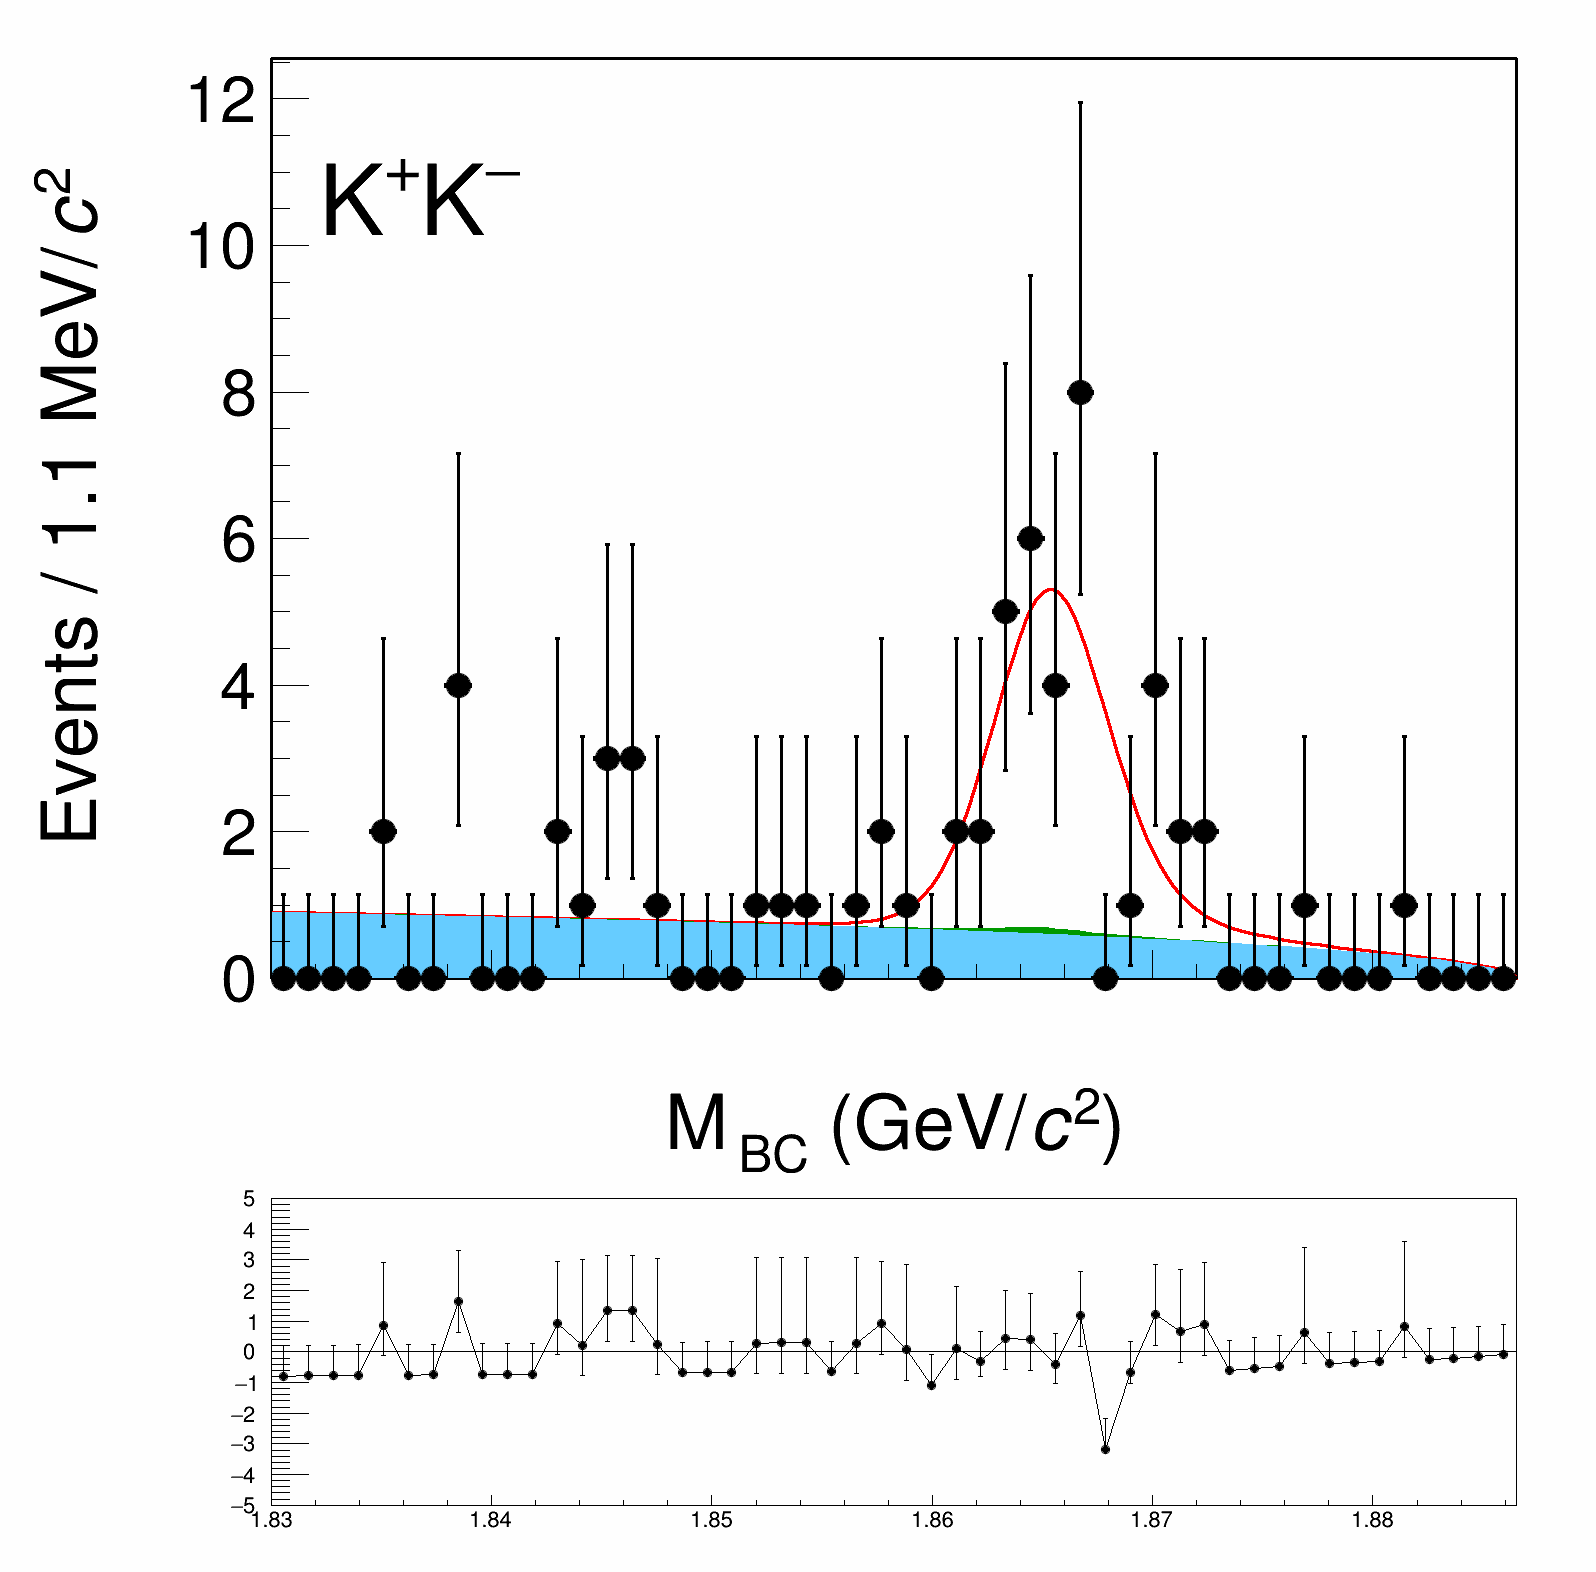
\includegraphics[height=4.2cm,trim={1.0cm 13.5cm 2.5cm 1.5cm},clip]{Plots/DoubleTagYield_DoubleTag_CP_KKpipi_vs_KK_SignalBin0.png}
    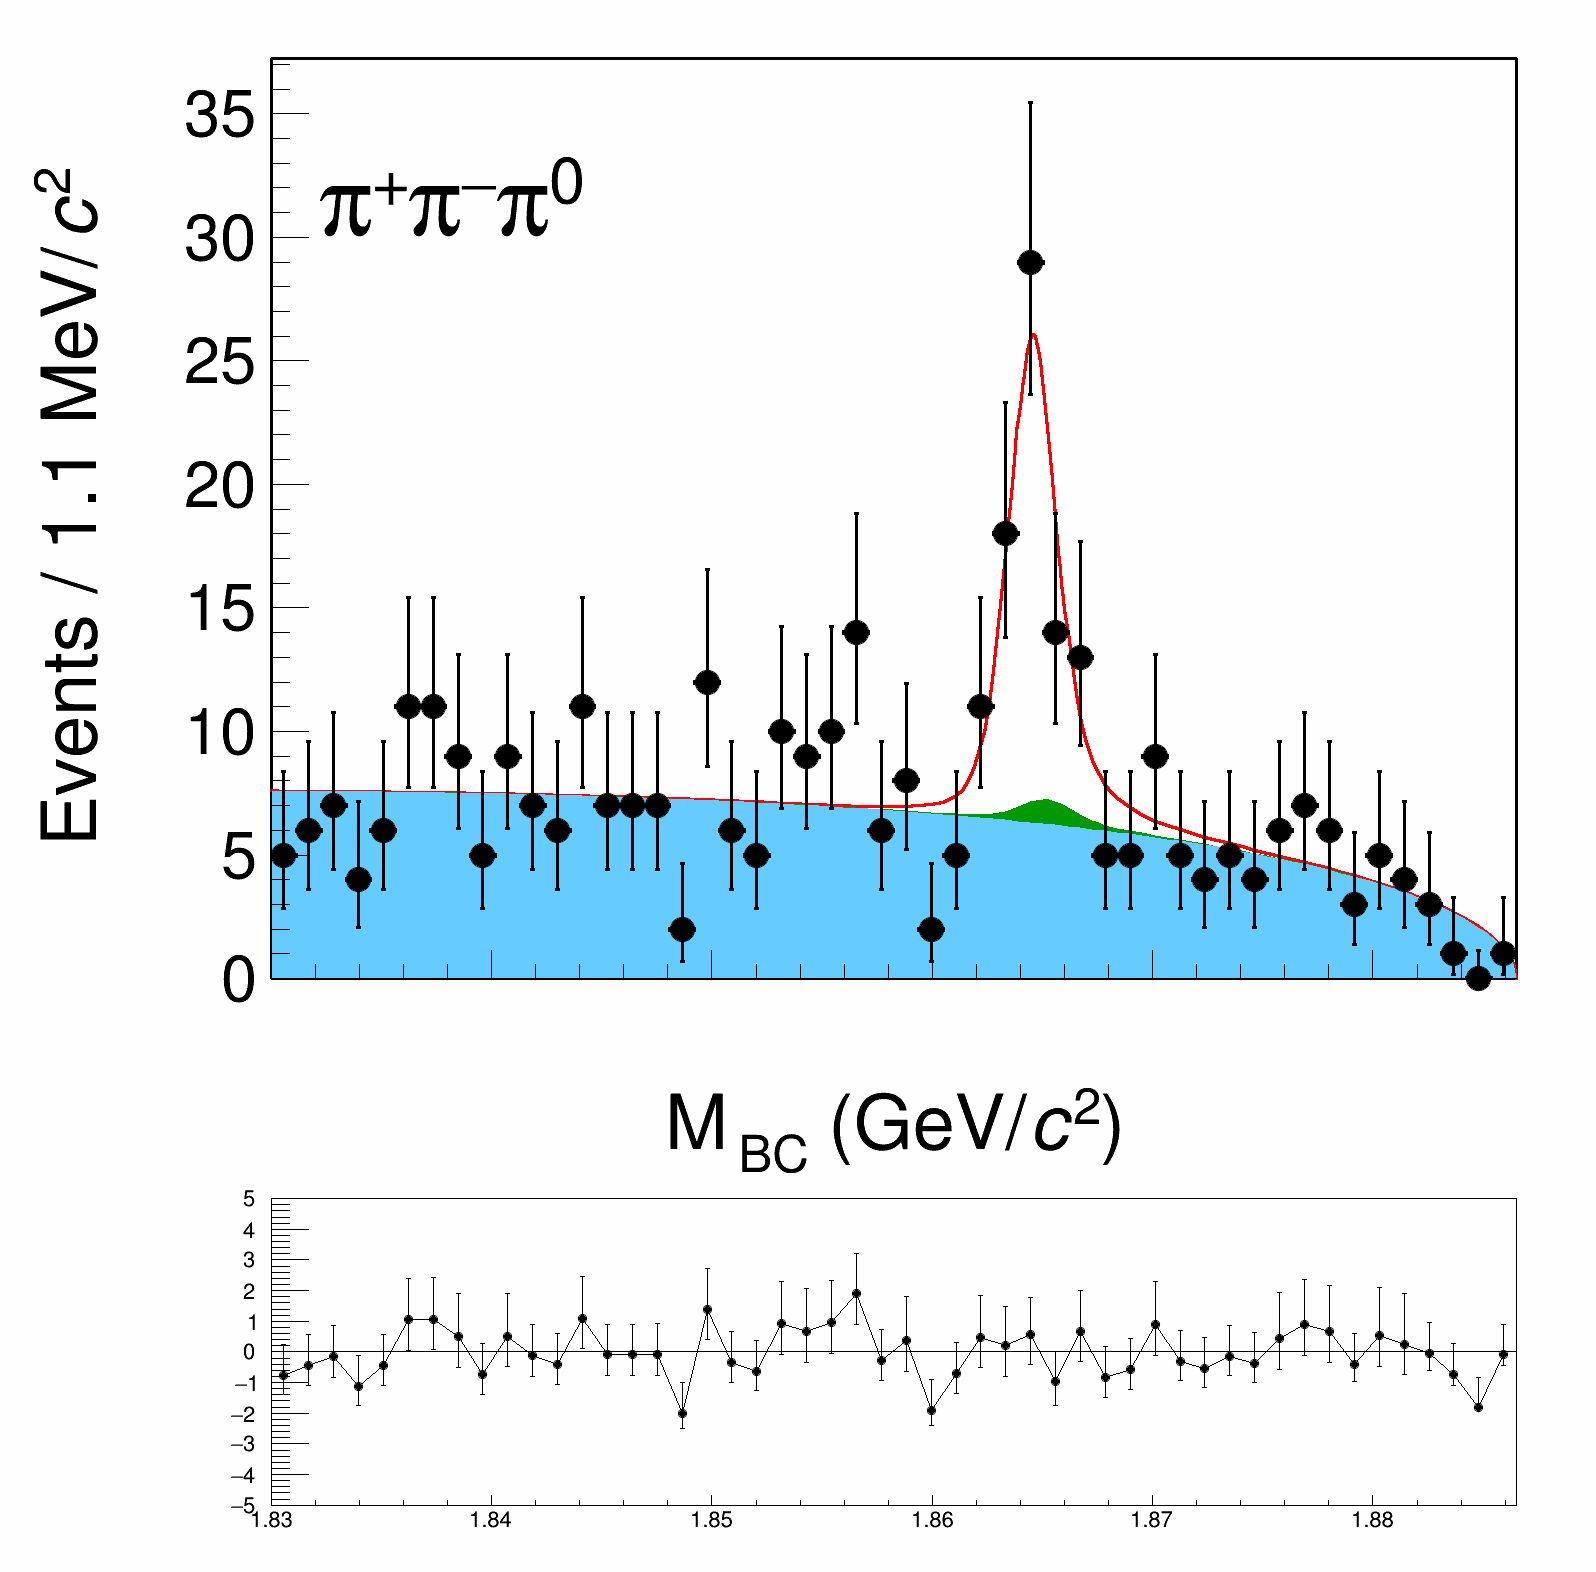
\includegraphics[height=4.2cm,trim={5.5cm 13.5cm 2.5cm 1.5cm},clip]{Plots/DoubleTagYield_DoubleTag_CP_KKpipi_vs_pipipi0_SignalBin0.png}
    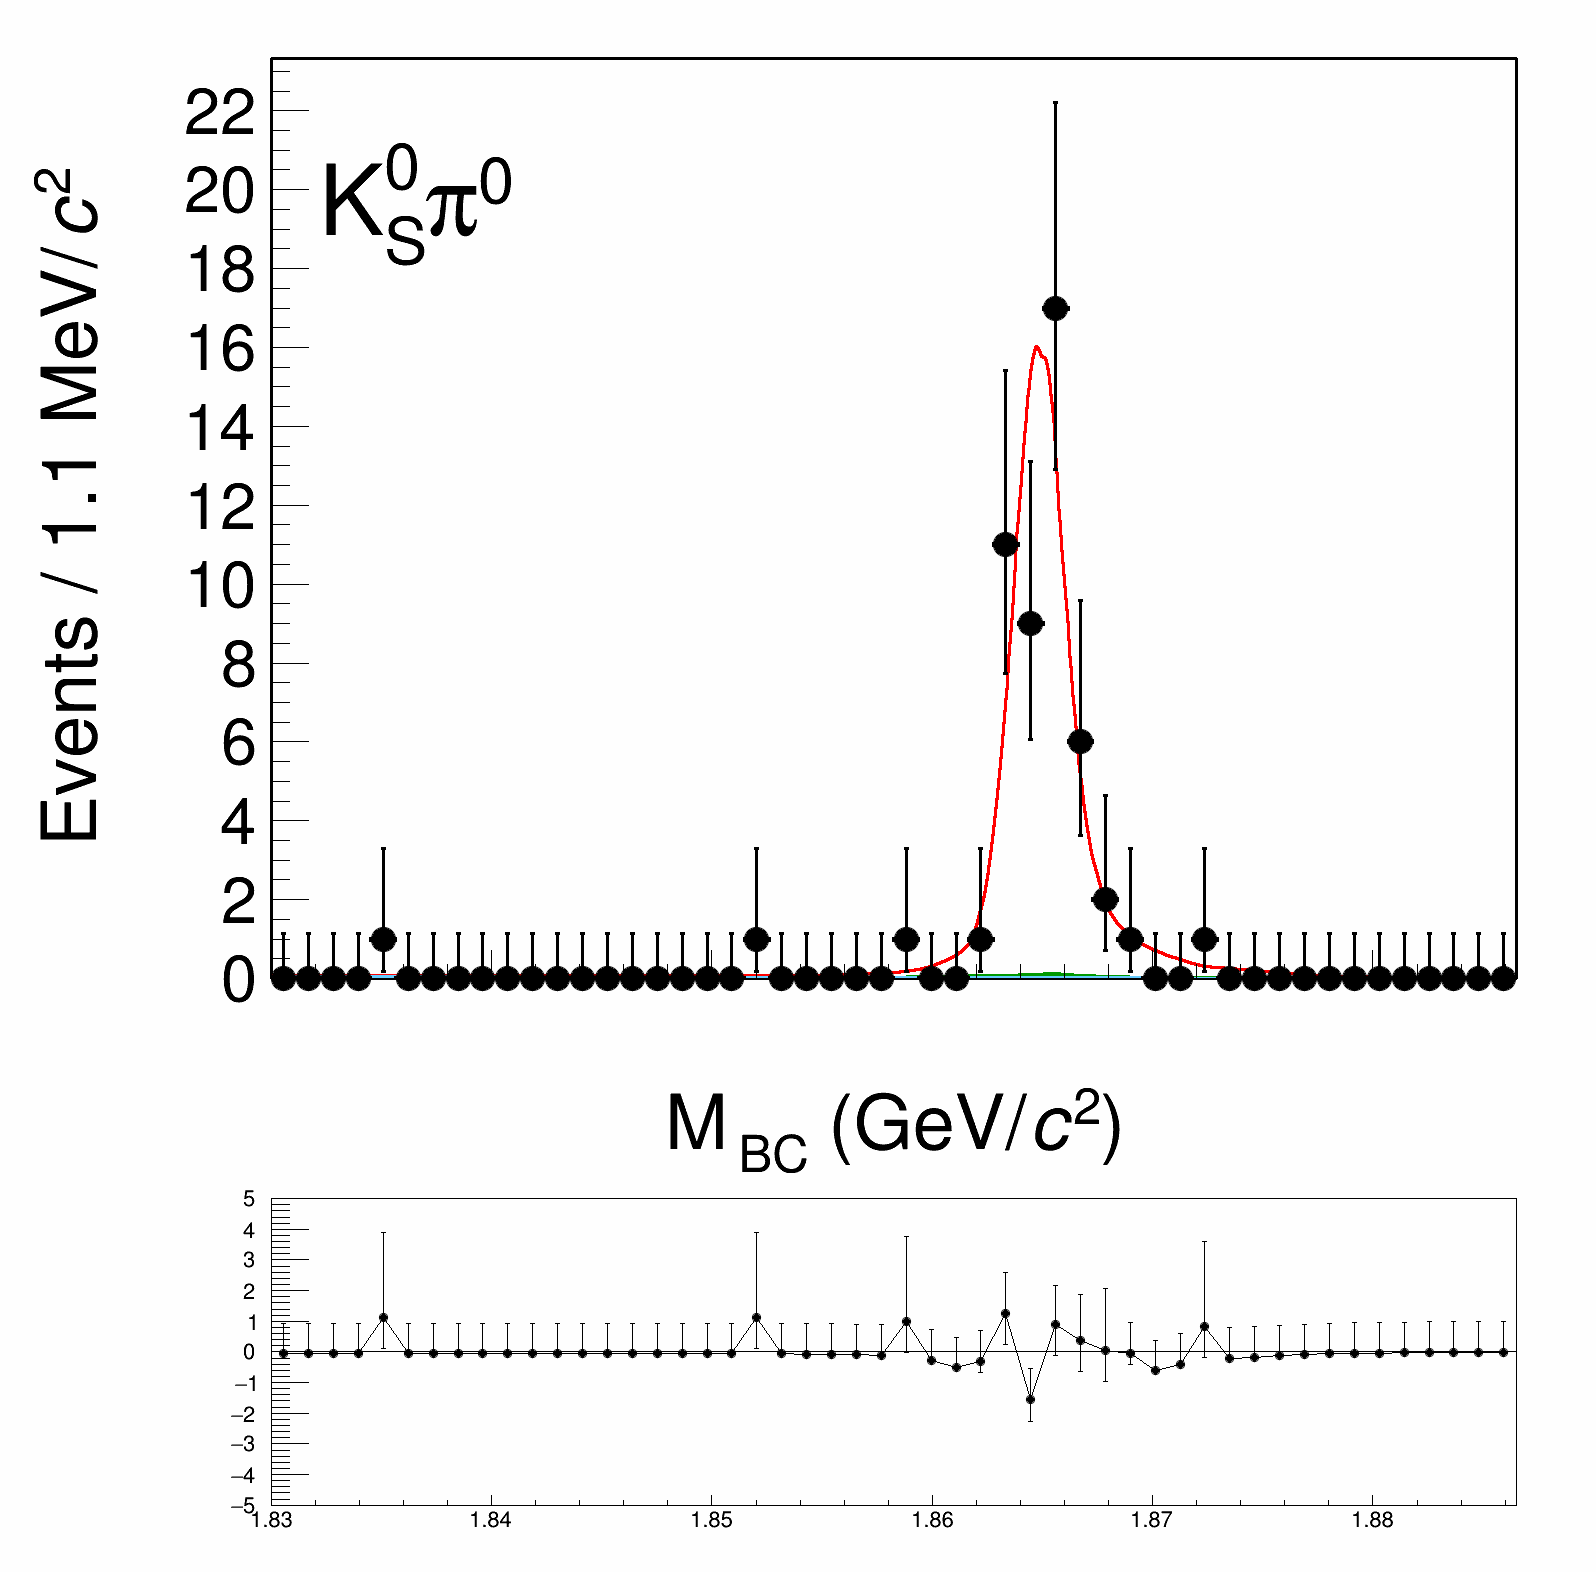
\includegraphics[height=4.2cm,trim={5.5cm 13.5cm 2.5cm 1.5cm},clip]{Plots/DoubleTagYield_DoubleTag_CP_KKpipi_vs_KSpi0_SignalBin0.png}
    \caption{DT $M_{\rm BC}$ distributions of fully reconstructed DT candidates. Data points are shown in black with error bars and the red curve is the fit result. The solid blue shape is combinatorial background. The green, stacked on top of the blue, is peaking background.}
    \label{figure:DT_MBC}
\end{figure*}

%%%%%%%%%%%%%%%%%%%%%%%%%%%%%%%%%%%%%%%%%%%%%%%%%%%%%%%%%%%%%%%
\subsection{Strong-phase fit}
\noindent Because of the statistically limited size of the BESIII dataset, the analysis is initially performed inclusively to determine the $C\!P$-even fraction $F_+$ of $D^0\to K^+K^-\pi^+\pi^-$. A maximum-likelihood fit is performed to the phase space inclusive ST and DT yields of $C\!P$ tags, assuming the relation given by Eq.~\eqref{equation:DT_ST_yield_ratio_FPlus}. The branching fraction $\mathcal{B}(KK\pi\pi)$ and the $C\!P$-even fraction $F_+$ are free parameters in the fit. Figure~\ref{figure:FPlus_CP_tags} shows the ratio of DT yields to ST yields for each tag after efficiency corrections. Physically, this represents the effective branching fraction of $D\to K^+K^-\pi^+\pi^-$, where the $D$ meson is prepared in a $C\!P$ eigenstate. The fitted $C\!P$-even fraction is $F_+ = 0.704 \pm 0.042 \pm 0.028$, where the first uncertainty is from the statistical uncertainties of ST and DT yields and the second uncertainty is the systematic uncertainty. The obtained branching fraction is $\mathcal{B}(KK\pi\pi) = (2.8 \pm 0.3)\times 10^{-3}$, where the uncertainty is statistical. It is consistent with the current value from the Particle Data Group (PDG)~\cite{pdg}.

There are several sources of systematic uncertainty, but most of these are very small. The dominant systematic is the knowledge of the $K^0_L\pi^0$ ST yield, which is limited by the $K^0_L\pi^0$ branching fraction uncertainty.

\begin{figure*}[htb]
    \centering
    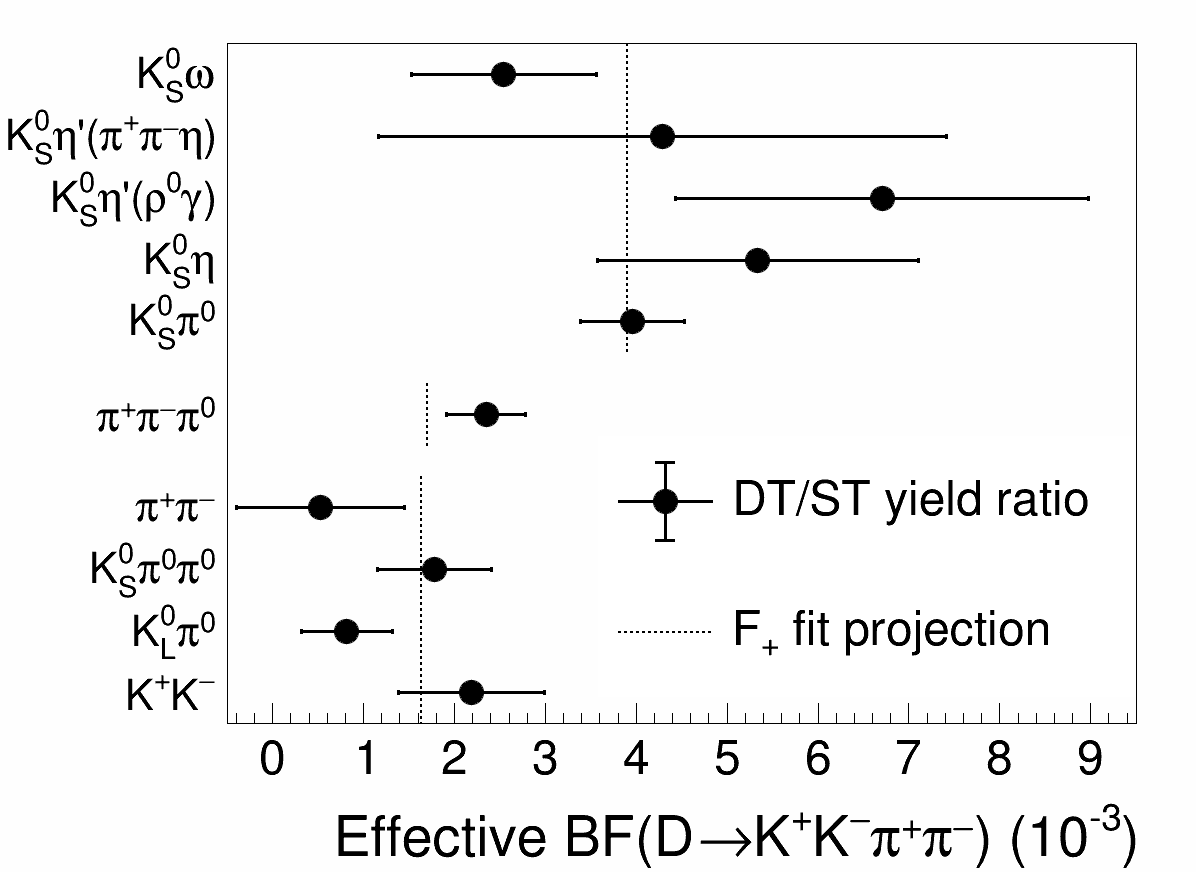
\includegraphics[width=0.5\textwidth]{Plots/CPeven_fraction_combination_CPtags.png}
    \caption{The branching fraction of $D\to K^+K^-\pi^+\pi^-$ measured with $C\!P$-odd (top) and $C\!P$-even (bottom) tags. The black dotted lines indicate the values expected from the fit.}
    \label{figure:FPlus_CP_tags}
\end{figure*}

A similar fit is performed for the modes $K^0_{S, L}\pi^+\pi^-$, using the relation in Eq.~\eqref{equation:DT_ST_yield_ratio_K0pipi_FPlus}, and the result is $F_+ = 0.798 \pm 0.077 \pm 0.019$. This is consistent with the $C\!P$ tags and combined, the final measurement of the $C\!P$-even fraction is $F_+ = 0.730 \pm 0.037 \pm 0.021$. This is the first measurement of $F_+$ in this channel.

In 2022, $\SI{5}{\per\femto\barn}$ of $\psi(3770)$ was successfully collected at BESIII, bringing the total dataset to $\SI{8}{\per\femto\barn}$. Using the same selection on this larger dataset, a first measurement of $c_i$ and $s_i$ will be performed. The yield determination will follow an identical strategy and the strong-phase fit will use Eqs.~\eqref{equation:DT_ST_yield_ratio} and \eqref{equation:DT_ST_yield_ratio_K0pipi}.

%%%%%%%%%%%%%%%%%%%%%%%%%%%%%%%%%%%%%%%%%%%%%%%%%%%%%%%%%%%%%%%
\section{Analysis of \texorpdfstring{\boldmath{$B^\pm\to[K^+K^-\pi^+\pi^-]_Dh^\pm$}}{B2DhD2KKpipi} at LHCb}
\subsection{The LHCb detector}
\noindent LHCb \cite{LHCb-DP-2008-001} is a single arm forward spectrometer designed to study beauty and charm hadrons in $pp$ collisions. The components important for this analysis are the tracking system and the Ring Imaging Cherenkov counters (RICH1 and RICH2). The tracking system includes the Vertex Locator (VELO), which provide high precision tracking and identification of displaced secondary vertices. A dipole magnet and the tracking stations measure charged particle momenta. The RICH detectors provides identification of kaons and pions. A $\SI{9}{\per\femto\barn}$ dataset at $\sqrt{s} = 7$, $8$ and $\SI{13}{\tera\eV}$ will be used in this analysis.

%%%%%%%%%%%%%%%%%%%%%%%%%%%%%%%%%%%%%%%%%%%%%%%%%%%%%%%%%%%%%%%
\subsection{\texorpdfstring{\boldmath{$B^\pm\to[K^+K^-\pi^+\pi^-]_Dh^\pm$}}{B2DhD2KKpipi} candidate selection}
\label{section:Candidate_selection}
\noindent A $B^\pm$ candidate is reconstructed by combining five charged tracks. Four of the charged tracks are required to have an invariant mass within $\SI{25}{\mega\eV/c^2}$ of the $D^0$ meson mass~\cite{pdg}. This requirement, which corresponds to around two and a half times the resolution of the mass peak, removes processes that have either a missing or misidentified particle.

Candidates where the opening angle between any pair of tracks from the $D$-decay products is smaller than $0.03^\circ$ are discarded, as these are likely to be hits from a single charged particle that is duplicated in the reconstruction. To suppress charmless background, which arises from $B^\pm$ meson decays where there is no intermediate charm meson, the distance between the $D$ and $B^\pm$ decay vertices is required to be greater than twice its resolution. This criterion eliminates $95\%$ of this category of decays.

Separation of $B^\pm\to DK^\pm$ and $B^\pm\to D\pi^\pm$ decays is achieved by imposing mutually exclusive particle identification (PID) requirements on the companion track, which is the $K^\pm$ or $\pi^\pm$ meson of the $B^\pm\to Dh^\pm$ decay. Companion tracks that have associated activity in the muon detector are removed; this requirement reduces background from semi-leptonic $b$-hadron decays involving a muon which is misidentified as a companion kaon or pion. The corresponding background from electrons is found to be negligible.  

Background from $D$ decays where a $\pi^+\pi^-$ pair originates from a $K^0_S$ meson is suppressed by excluding regions containing $\pi^+\pi^-$ pairs with invariant mass inside the interval $[477, 507]\si{\mega\eV/c^2}$ from the binning scheme. Additionally, PID requirements are imposed on the kaon from the $D$ candidate with opposite sign to the companion track. This selection requirement suppresses $D\to K^\mp\pi^\pm\pi^-\pi^+\pi^0$ background where the $\pi^0$ meson is not reconstructed and the kaon is misidentified. 

Combinatorial background is suppressed using a boosted decision tree~(BDT). Simulated signal events are used as the signal training sample, while candidates in the far upper $B^\pm$ sideband between $5800$-$7000\si{\mega\eV/c^2}$ form the background training sample. The input variables of the BDT include information on the momenta and impact parameters of the $B^\pm$, $D$ and companion-track candidates. The optimal working point of the BDT is determined by performing pseudoexperiments to determine the cut value that provides the best sensitivity to $\gamma$. Candidates with a BDT score below this cut value are discarded.

To improve the resolution of the momenta of the $D$-decay products and the invariant mass of the $B^\pm$ candidate, a kinematic fit is performed in which the $D$ meson candidate is constrained to its known mass~\cite{pdg}, and the $B^\pm$ candidate is required to originate from its PV. This is defined as the PV with the smallest impact parameter.

%%%%%%%%%%%%%%%%%%%%%%%%%%%%%%%%%%%%%%%%%%%%%%%%%%%%%%%%%%%%%%%
\section{\texorpdfstring{\boldmath{$B^\pm\to[K^+K^-\pi^+\pi^-]_Dh^\pm$}}{B2DhD2KKpipi} global mass fit and binned CP fit}
\noindent An unbinned, extended maximum-likelihood fit is performed to the invariant-mass spectrum of the $B^\pm\to[K^-K^+\pi^+\pi^+]_Dh^\pm$ candidates in the range from $\SI{5080}{\mega\eV/c^2}$ to $\SI{5700}{\mega\eV/c^2}$. The fit is first performed on the $B^\pm\to DK^\pm$ and $B^\pm\to D\pi^\pm$ candidates, integrated over all phase-space bins, which is referred to as the global fit. The global fit is used to determine the parameters of the functions that describe the signal and background invariant-mass distributions. The $B^\pm\to[K^-K^+\pi^+\pi^-]_Dh^\pm$ invariant-mass distributions are shown in Fig.~\ref{figure:Global_fit}.

The yield of $B^\pm\to D\pi^\pm$ is varied separately for the two $D$ decays, while the yield of $B^\pm\to DK^\pm$ is parameterised as a ratio relative to the $B^\pm\to D\pi^\pm$ yield. This ratio is a common fit parameter, as are the parameters that describe the signal shape.

\begin{figure}[htb]
    \centering
    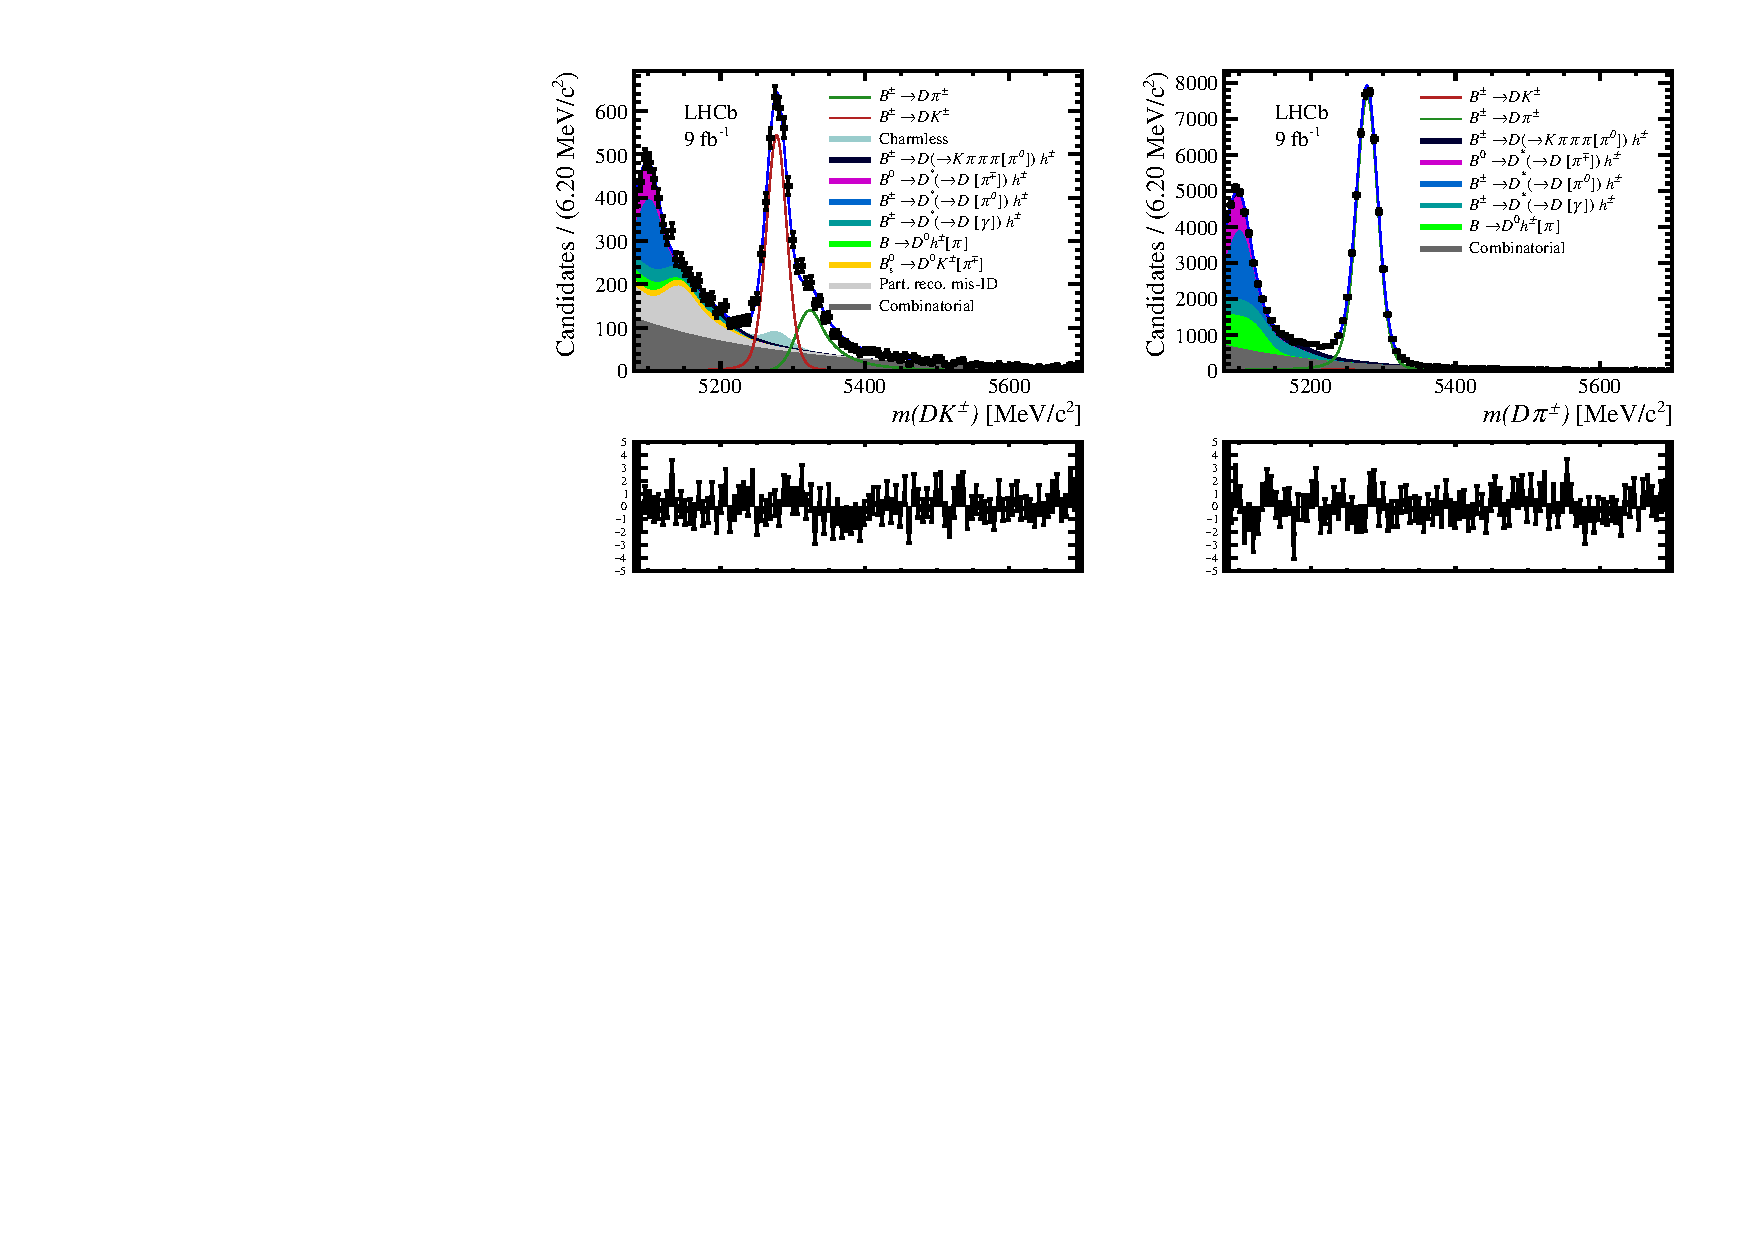
\includegraphics[width=1.0\textwidth,trim={0 2.9cm 0 0},clip]{Plots/d2kkpipi_fiveL_allDP.pdf}
    \caption{Invariant-mass distributions for the (left) $B^\pm\to DK^\pm$ selection and (right) $B^\pm\to D\pi^\pm$ selection, with $D\to K^+K^-\pi^+\pi^-$. The data is shown as black points and the blue curve is the fit result. The square brackets in the legend denote particles that are not reconstructed.}
    \label{figure:Global_fit}
\end{figure}

The signal peak at around $\SI{5280}{\mega\eV/c^2}$ corresponds to correctly reconstructed $B^\pm\to[K^+K^-\pi^+\pi^-]_Dh^\pm$ candidates. The signal invariant-mass shape is parameterised as
\begin{equation}
    \begin{aligned}
        f_{\rm signal}(m|m_B, \sigma, \alpha_L, \alpha_R, \beta, k) =& k\times f_{\rm MG}(m|m_B, \sigma, \alpha_L, \alpha_R, \beta) \\
                                                                     +& (1 - k)\times f_{\rm G}(m|m_B, \sigma),
    \end{aligned}
\end{equation}
where $f_{\rm G}$ is a Gaussian function and $f_{\rm MG}$ is a modified Gaussian function,

\begin{equation}
    f_{\rm MG}(m|m_B, \sigma, \alpha_L, \alpha_R, \beta)\propto
    \begin{cases}
        \exp\Big(-\frac{\Delta m^2(1 + \beta\Delta m^2)}{2\sigma^2 + \alpha_L\Delta m^2}\Big), \quad \Delta m = m - m_B < 0, \\
        \exp\Big(-\frac{\Delta m^2(1 + \beta\Delta m^2)}{2\sigma^2 + \alpha_R\Delta m^2}\Big), \quad \Delta m = m - m_B > 0.
    \end{cases}
\end{equation}
The function $f_{\rm MG}$ has approximately Gaussian behaviour when $\Delta m^2\ll\sigma^2/\alpha_{L, R}$ or $\Delta m^2\gg\beta^{-1}$, but it has tails that model the experimental resolution. The tail parameters $\alpha_{L, R}$ and $\beta$, and the fraction $k$, are determined in a fit to simulated events, but the peak position $m_B$ and the width $\sigma$ are determined in the fit to data. The mass $m_B$ is common between the $B^\pm\to DK^\pm$ and $B^\pm\to D\pi^\pm$ channels, but $\sigma$ is different because the $B^\pm\to DK^\pm$ width is narrower due to the lower energy release in the decay.

At masses above the $B^\pm\to DK^\pm$ peak there is a non-negligible contribution from $B^\pm\to D\pi^\pm$ decays where the companion is misidentified as a kaon. The rate of this cross-feed background is fixed from the relative PID efficiencies, which are determined in calibration data that is weighted to match the momentum and pseudorapidity distributions of the companion track of the signal. The exact shape is determined using a data-driven method by swapping the mass hypothesis of the companion track in the $B^\pm\to D\pi^\pm$ peak. Similarly, the shape of $B^\pm\to DK^\pm$ candidates misidentified as $B^\pm\to D\pi^\pm$ candidates is also accounted for, but the impact of this background is minimal due to its smaller branching fraction.

Candidates with masses below that of the signal peak are background from $B$-meson decays where a neutral particle or charged pion is not reconstructed. This partially reconstructed background is parameterised using a model developed in Ref.~\cite{LHCb-PAPER-2020-019}.

Additionally, the decay $D\to K^+K^-\pi^+\pi^-$ is also contaminated by $D\to K^\mp\pi^\pm\pi^-\pi^+\pi^0$ decays, where a charged pion is misidentified as a kaon and the neutral pion is not reconstructed. This background is present below the signal peak, but it has a large tail towards the upper end of the invariant mass spectrum of the $B^\pm$ candidates. The shape of this background is fixed using a simulation sample, while the yield is a free parameter.

The contamination of charmless decays in the $D\to K^+K^-\pi^+\pi^-$ mode is also different from Ref.~\cite{LHCb-PAPER-2020-019}. In particular, the $B^\pm\to[K^+K^-\pi^+\pi^-]_DK^\pm$ sample has a significant contribution from the mode $B^\pm\to K^+K^-\pi^+\pi^-K^\pm$. Both the magnitude and invariant-mass shape of this contribution are fixed in the invariant-mass fit from studies of the lower sideband of the invariant $D$ mass. Analogous studies show that there are no significant contamination from charmless decays in the $B^\pm\to D\pi^\pm$ selection.

From the global fit, it was found that the signal yield is $\SI{3026(38)}{}$ for $B^\pm\to DK^\pm$ and $\SI{44349(218)}{}$ for $B^\pm\to D\pi^\pm$. After the global invariant-mass fit, a second fit is performed where the $B^\pm\to DK^\pm$ and $B^\pm\to D\pi^\pm$ candidates are split by charge and sorted into bins of phase space, which makes a total of $2\times 2\times 16 = 64$ categories. The lower fit boundary is increased to $\SI{5150}{\mega\eV/c^2}$ to remove most of the partially reconstructed background. The shape parameters and relative yields of the different background components are fixed from the global fit. The signal yields in each bin are parameterised in terms of the $C\!P$-violating observables, which are free parameters in the fit. The $F_i$ parameters are also free parameters, while the strong-phase parameters $c_i$ and $s_i$ are fixed according to the LHCb amplitude model.

In each bin, the yield of combinatorial background and partially reconstructed background are free parameters, with the exception of the $B^0_s\to\bar{D^0}K^-\pi^+$ contamination, which is treated separately because the charm meson has the flavour opposite to the signal decay and the other partially reconstructed backgrounds. In $B^-$ ($B^+$) decays, the fractional bin yield of the $B^0_s$ ($\bar{B^0_s}$) background is therefore set equal to $F_{-i}$ ($F_i$).

The distribution of charmless background between phase-space bins is determined from the lower $D$-mass sideband. The distribution of $D\to K^\mp\pi^\pm\pi^-\pi^+\pi^0$ decays between bins is assumed to be proportional to the bin volume, since studies of simulation samples show that these decays are approximately uniform in the $D\to K^+K^-\pi^+\pi^-$ phase space.

The fitted $C\!P$-violating observables are listed in Table~\ref{table:GGSZ_observables} and plotted in Fig.~\ref{figure:CP_observables}, along with the likelihood contours, which only include statistical uncertainties. The lengths of the two vectors from the origin to $(x_\pm^{DK}, y_\pm^{DK})$ determine $r_B^{DK}$, while the angle between them is $2\gamma$. In the absence of $C\!P$ violation, the two vectors would be identical. The vector from the origin to $(x_\xi^{D\pi}, y_\xi^{D\pi})$ indicates the relative size and angle between $r_B$ and $\delta_B$ of the $B^\pm\to D\pi^\pm$ and $B^\pm\to DK^\pm$ decays. Since this contour overlaps with the origin, the sensitivity to $C\!P$ violation is much smaller in the $B^\pm\to D\pi^\pm$ mode.

\begin{table}[htb]
    \centering
    \caption{$C\!P$-violating observables of the binned measurement, multiplied by $10^2$.  The first uncertainty is statistical, the second is systematic, and the third is associated with the model dependence of the strong-phase parameters.}
    \label{table:GGSZ_observables}
    \begin{tabular}{cc} 
        \toprule
        $C\!P$-violating observable & Fit result ($\times 10^2$)           \\
        \midrule
        $x_-^{DK}$      & \phantom{+}$7.9 \pm 2.9 \pm 0.4 \pm 0.4$        \\
        $y_-^{DK}$      & $-3.3 \pm 3.4 \pm 0.4 \pm 3.6$       \\
        $x_+^{DK}$      & $-12.5 \pm 2.5 \pm 0.3 \pm 1.7$\phantom{0}      \\
        $y_+^{DK}$      & $-4.2 \pm 3.1 \pm 0.3 \pm 1.3$ \\
        $x_\xi^{D\pi}$    & $-3.1 \pm 3.5 \pm 0.7 \pm 0.1$       \\
        $y_\xi^{D\pi}$    & $-1.7 \pm 4.7 \pm 0.6 \pm 1.1$       \\
        \bottomrule
    \end{tabular}
\end{table}

\begin{figure}[htb]
    \centering
    \begin{subfigure}{0.5\textwidth}
        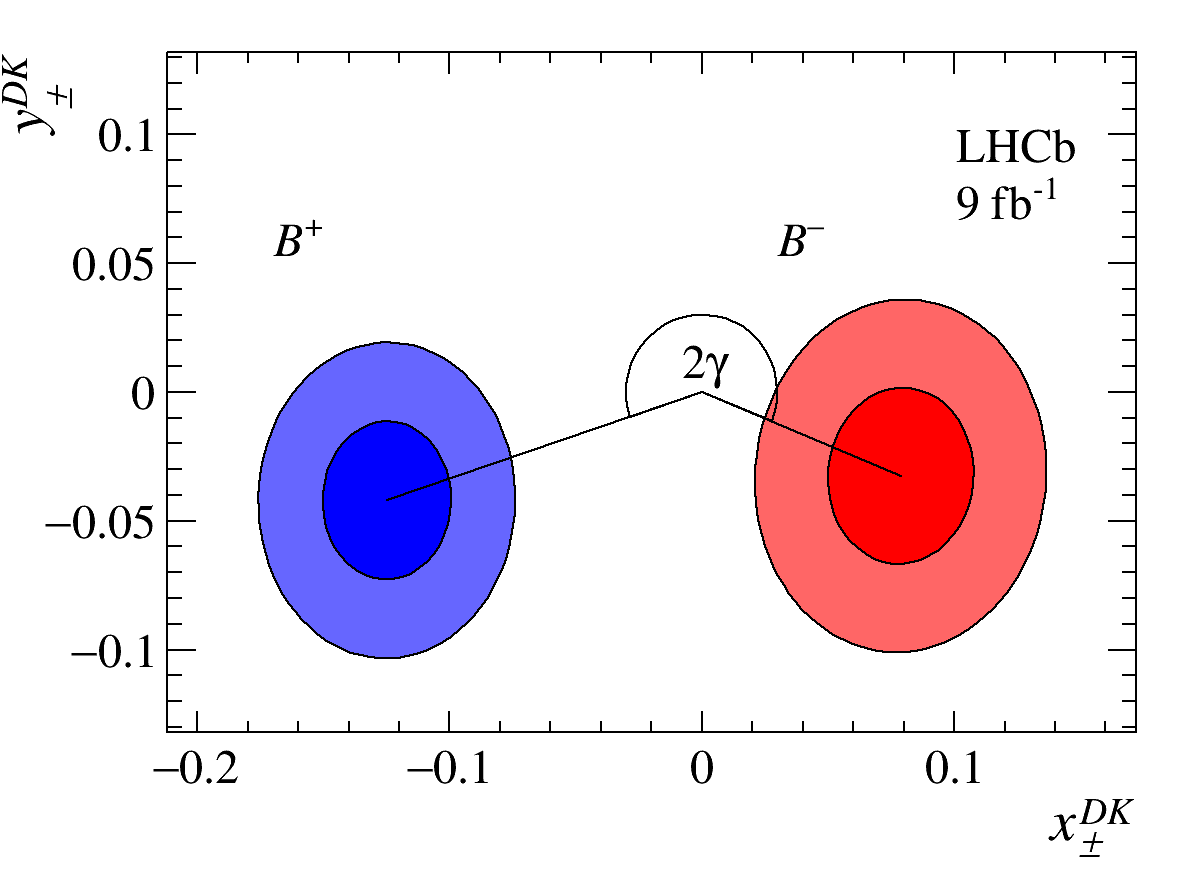
\includegraphics[width=1\textwidth]{Plots/B2DK_CP_Observables_Contours.png}
        \caption{$B^\pm\to DK^\pm$.}
        \label{figure:CP_observables_DK}
    \end{subfigure}%
    \begin{subfigure}{0.5\textwidth}
        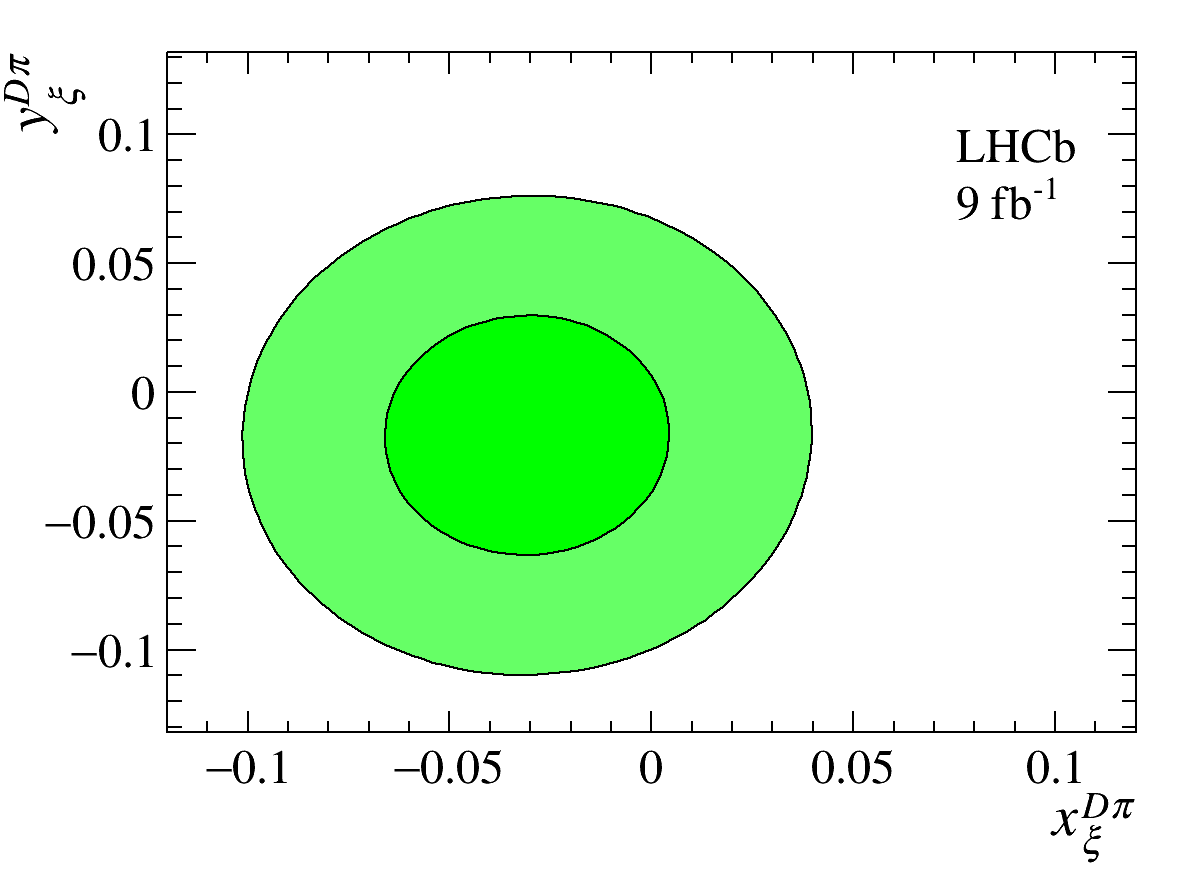
\includegraphics[width=1\textwidth]{Plots/B2Dpi_CP_Observables_Contours.png}
        \caption{$B^\pm\to D\pi^\pm$.}
        \label{figure:CP_observables_Dpi}
    \end{subfigure}
    \caption{Graphical representation of the $C\!P$-violating observables. The $1\sigma$ and $2\sigma$ contours, which represent the statistical uncertainties, are also shown. On the left, the blue (red) contours belong to the $C\!P$-violating observables of the $B^+\to DK^+$ ($B^-\to DK^-$) decay, while on the right the green contours represent the $(x_\xi^{D\pi}, y_\xi^{D\pi})$ observables of the $B^\pm\to D\pi^\pm$ decay mode.}
    \label{figure:CP_observables}
\end{figure}

\begin{figure}[htb]
    \centering
    \begin{subfigure}{0.5\textwidth}
        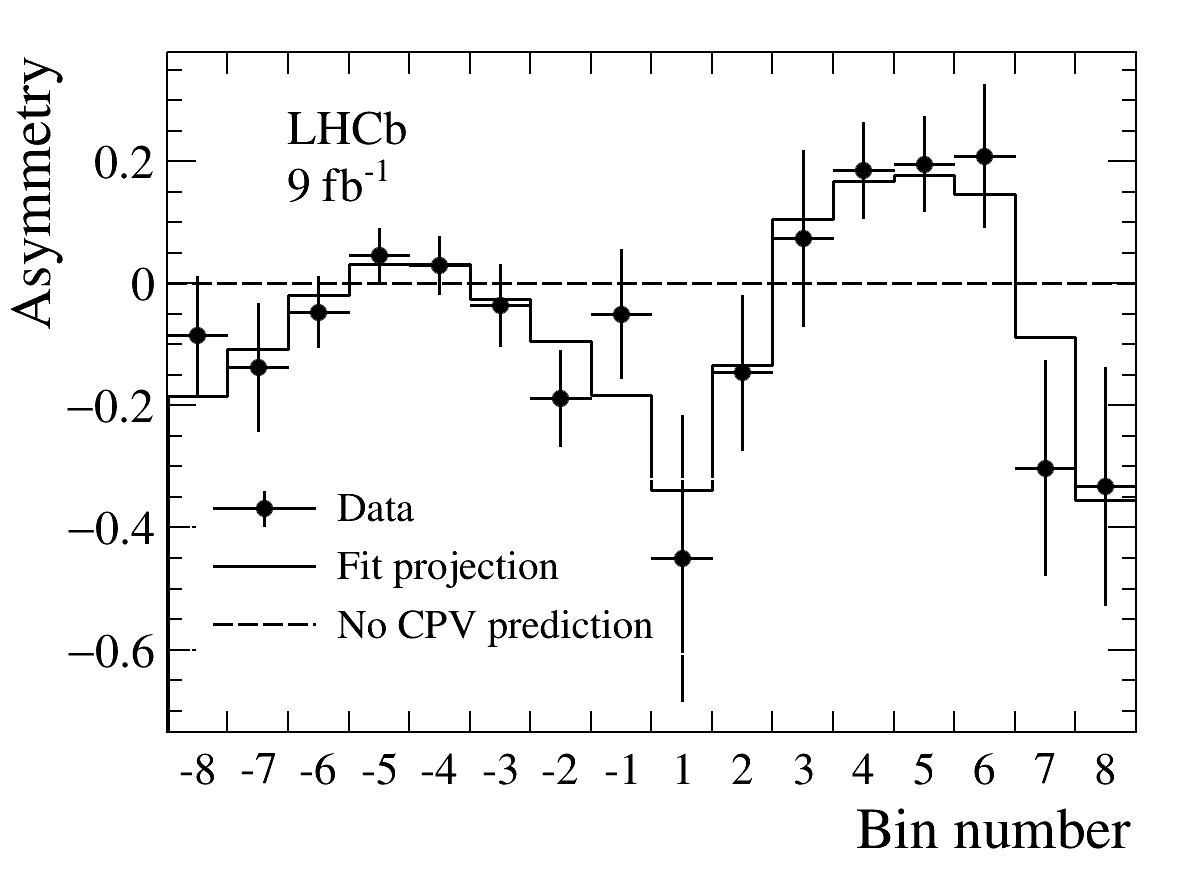
\includegraphics[width=1\textwidth]{Plots/BinAsymmetries_dk.png}
        \caption{$B^\pm\to DK^\pm$.}
        \label{figure:Bin_asymmetries_DK}
    \end{subfigure}%
    \begin{subfigure}{0.5\textwidth}
        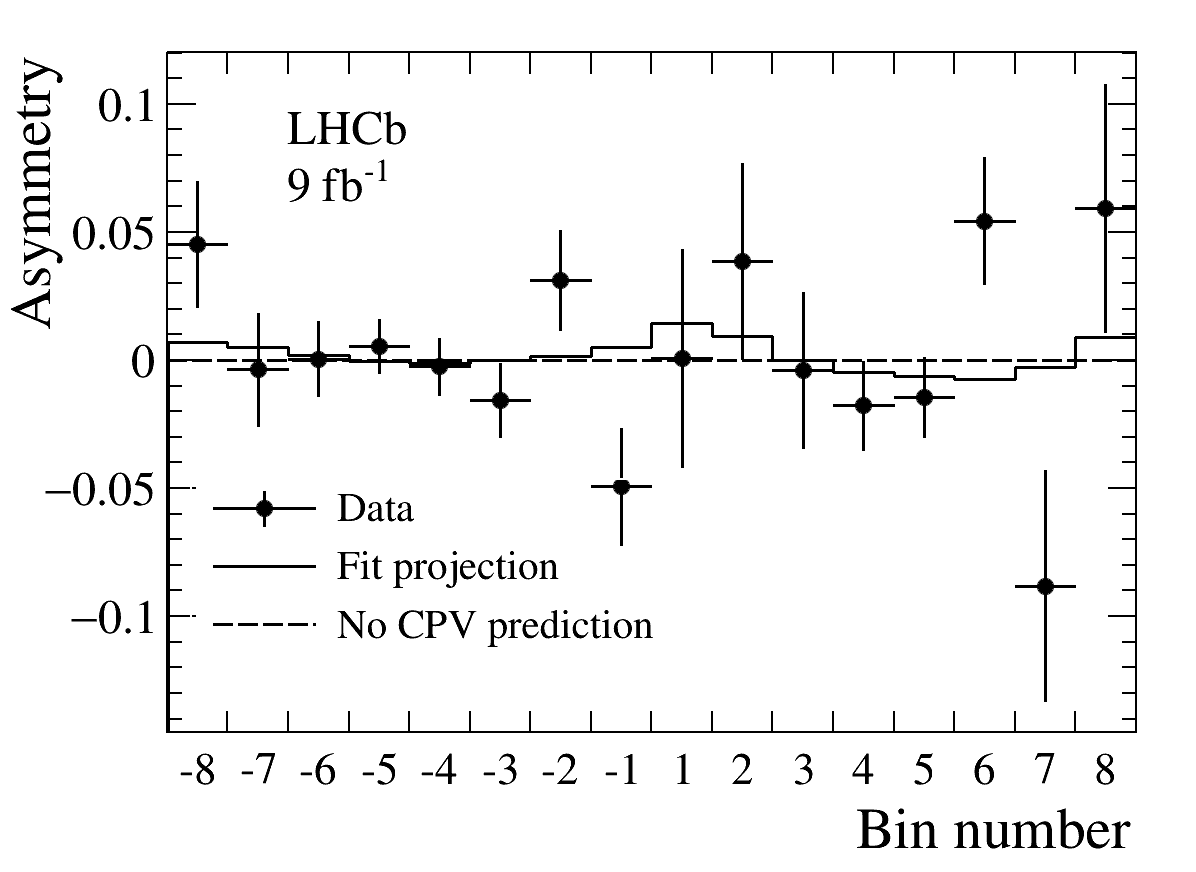
\includegraphics[width=1\textwidth]{Plots/BinAsymmetries_dpi.png}
        \caption{$B^\pm\to D\pi^\pm$.}
        \label{figure:Bin_asymmetries_Dpi}
    \end{subfigure}
    \caption{The $B^\pm\to[K^+K^-\pi^+\pi^-]_D h^\pm$ fractional bin asymmetries in each phase-space bin. The solid black line is the prediction using the fitted $C\!P$-violating observables. The dashed line indicates the asymmetry prediction in the absence of $C\!P$ violation.}
    \label{figure:Bin_asymmetries}
\end{figure}

In Table~\ref{table:GGSZ_observables}, the first uncertainty is statistical, the second is the internal LHCb systematic uncertainty and the third is the systematic uncertainty associated with the model. The internal systematic uncertainties are generally small and they are similar to that described in Ref.~\cite{LHCb-PAPER-2020-019}. To evaluate the model systematic uncertainty, pseudoexperiments are generated using strong-phases from an older amplitude model~\cite{CLEO_KKpipi_cisi} and fitted back using the nominal values of $c_i$ and $s_i$. The shift in the central values are taken as the systematic uncertainty associated with the model dependence.

The $C\!P$-violation effects can be illustrated directly by considering the asymmetries in each bin. This information is obtained from an alternative fit where the signal yields, instead of the $C\!P$-violating observables, are determined. The bin asymmetries, $(N_i^- - N_{-i}^+)/(N_i^- + N_{-i}^+)$, calculated from these yields are shown in Fig.~\ref{figure:Bin_asymmetries}. The bin yields are normalised separately for $B^-$ and $B^+$, so that only bin-to-bin variations are apparent. Some of those for $B^\pm\to DK^\pm$ are significant, and exhibit a non-trivial distribution, which is driven by the variation in the strong-phase difference between $D^0$ and $\bar{D^0}$ decays. In the $B^\pm\to D\pi^\pm$ mode, there is a lower sensitivity to $C\!P$ violation and therefore no such behaviour is seen. Although the results shown in Fig.~\ref{figure:CP_observables} depend on strong-phases predicted from an amplitude model, the $C\!P$-violation seen in Fig.~\ref{figure:Bin_asymmetries_DK} are model-independent.

%%%%%%%%%%%%%%%%%%%%%%%%%%%%%%%%%%%%%%%%%%%%%%%%%%%%%%%%%%%%%%%
\section{Interpretation in terms of \texorpdfstring{\boldmath{$\gamma$}}{gamma}}
\noindent The $C\!P$-violating observables in Table~\ref{table:GGSZ_observables} can be expressed in terms of $\gamma$ and other physics parameters using Eq.~\eqref{equation:CP_observables}, using a maximum likelihood fit. The result is

\begin{align*}
    \gamma &= (116^{+12}_{-14})^\circ, \\
    \delta_B^{DK} &= (81^{+14}_{-13})^\circ, \\
    r_B^{DK} &= 0.110^{+0.020}_{-0.020}, \\
    \delta_B^{D\pi} &= (298^{+62}_{-118})^\circ, \\
    r_B^{D\pi} &= 0.0041^{+0.0054}_{-0.0041}.
\end{align*}
It should be stressed that currently the parameters from Table~\ref{table:GGSZ_observables} depend on model-predicted strong-phase parameters, which may have systematic uncertainties associated with the model that cannot be evaluated. It is therefore not unexpected that the value of $\gamma$ deviates from the world average by around $3\sigma$. In fact, it emphasises the importance of the ongoing model-independent measurement of $c_i$ and $s_i$.

%%%%%%%%%%%%%%%%%%%%%%%%%%%%%%%%%%%%%%%%%%%%%%%%%%%%%%%%%%%%%%%
\section{Conclusion and future work}
\noindent A first measurement of $\gamma$ in the channel $B^\pm\to[K^+K^-\pi^+\pi^-]_Dh^\pm$ has been presented. The measurement combines a strong-phase analysis of the $D$-meson decay from BESIII and a $C\!P$-violation study of $B^\pm\to Dh^\pm$ from LHCb. This measurement will complement the current set of $\gamma$ measurements using other $B$-decay modes. In addition, the strong-phase measurements of the $D$ decay will provide important inputs for $D^0$-$\bar{D^0}$ mixing and charm $C\!P$ violation studies.

%%%%%%%%%%%%%%%%%%%%%%%%%%%%%%%%%%%%%%%%%%%%%%%%%%%%%%%%%%%%%%%                                                                          
\bibliography{references}
%\bibliographystyle{unsrt}
\bibliographystyle{JHEP}

\end{document}